%% GENERATED by tools/from_docs.py from stepss-docs. Do not edit by hand:
%% edit the page named below in stepss-docs and regenerate.
%% source: stepss-docs/src/content/docs/models/ieee-exciters.md

\chapter{IEEE excitation controllers}\label{doc:model-exc-ieee}

These excitation system models implement the IEEE Std 421.5-2016 ``IEEE Recommended Practice for Excitation System Models for Power System Stability Studies'' (and selected ENTSO-E variants) within RAMSES. Each model is defined using the CODEGEN domain-specific language (DSL) and compiled into Fortran for time-domain simulation. The DSL describes block diagrams as interconnected transfer function primitives (\texttt{tf1p}, \texttt{tf1p1z}, \texttt{tf1plim}, \texttt{tfder1p}, \texttt{inlim}, \texttt{pictl}, etc.), initial conditions, and algebraic constraints, forming a self-contained, portable model definition.

\begin{docsnote}{Usage in Dynamic Data Files}

Exciter models in RAMSES are defined as sub-records within a \texttt{SYNC\_MACH} block using the \texttt{EXC} keyword, followed by the model name and its parameters. They are not standalone records. The \texttt{EXC} line appears after the machine parameters and before the \texttt{TOR} (torque/governor) line. The entire block ends with a single \texttt{;} after the \texttt{TOR} record.

\begin{Verbatim}
SYNC_MACH name bus FP FQ P Q SNOM Pnom H D IBRATIO
                    XT  Xl  Xd  X'd  X"d  Xq  X'q  X"q  m  n  Ra  T'do  T"do  T'qo  T"qo
              EXC model_name  param1  param2  ...
              TOR model_name  param1  param2  ... ;
\end{Verbatim}

RAMSES adds the \texttt{exc\_} prefix to the model name automatically, so both \texttt{AC1A} and \texttt{exc\_AC1A} are accepted.

The \textbf{State} column of the Model Index says whether a model is compiled and callable, or only a DSL description:

\begin{itemize}
\tightlist
\item
  \textbf{Registered}, callable from a data file as it stands. Every compiled exciter has been registered since 3.79; before that, fifteen of them were mapped to no name and RAMSES rejected them in a data file.
\item
  \textbf{DSL only}, present as a CODEGEN model description but not as compiled Fortran. \texttt{ENTSOE\_lim} ships as a ready-made example in the URAMSES \texttt{custom\_models/} directory; \texttt{AC8B\_lim} is listed for reference only and is not distributed.
\end{itemize}

The \hyperref[doc:model-index]{Model Reference index} carries the same information across all model families.

\end{docsnote}

\begin{center}\rule{0.5\linewidth}{0.5pt}\end{center}

\section{Model Index}\label{model-exc-ieee:model-index}

\begin{small}\begin{longtable}[]{@{}
  >{\raggedright\arraybackslash}p{(\linewidth - 12\tabcolsep) * \real{0.2433}}
  >{\raggedright\arraybackslash}p{(\linewidth - 12\tabcolsep) * \real{0.1605}}
  >{\raggedright\arraybackslash}p{(\linewidth - 12\tabcolsep) * \real{0.1750}}
  >{\raggedright\arraybackslash}p{(\linewidth - 12\tabcolsep) * \real{0.1053}}
  >{\raggedright\arraybackslash}p{(\linewidth - 12\tabcolsep) * \real{0.1145}}
  >{\raggedright\arraybackslash}p{(\linewidth - 12\tabcolsep) * \real{0.2013}}
@{}}
\toprule\noalign{}
\begin{minipage}[b]{\linewidth}\raggedright
Model Name
\end{minipage} & \begin{minipage}[b]{\linewidth}\raggedright
State
\end{minipage} & \begin{minipage}[b]{\linewidth}\raggedright
Base Type
\end{minipage} & \begin{minipage}[b]{\linewidth}\raggedright
PSS
\end{minipage} & \begin{minipage}[b]{\linewidth}\raggedright
OEL / Limiter
\end{minipage} & \begin{minipage}[b]{\linewidth}\raggedright
IEEE Reference
\end{minipage} \\
\midrule\noalign{}
\endhead
\bottomrule\noalign{}
\endlastfoot
\texttt{AC1A} & Registered & AC type 1 & & & IEEE 421.5 Type AC1A \\
\texttt{AC1A\_MAXEX2} & Registered & AC type 1 & & MAXEX2 field current limiter & IEEE 421.5 Type AC1A \\
\texttt{AC1A\_RETRO} & Registered & AC type 1 (retrofit) & PSS4B (internal) & & \\
\texttt{AC1A\_RETRO\_PSS4B} & Registered & AC type 1 (retrofit) & PSS4B & & \\
\texttt{AC4A} & Registered & AC type 4 & & & IEEE 421.5 Type AC4A \\
\texttt{AC8B} & Registered & AC type 8 & & & IEEE 421.5 Type AC8B \\
\texttt{AC8B\_PSS3B\_lim} & Registered & AC type 8 & PSS3B & Integral OEL + SCL & IEEE 421.5 Type AC8B \\
\texttt{AC8B\_lim} & DSL only & AC type 8 & & Integral OEL + SCL & IEEE 421.5 Type AC8B \\
\texttt{DC3A} & Registered & DC type 3 & & & IEEE 421.5 Type DC3A \\
\texttt{ENTSOE\_simp} & Registered & ENTSO-E simplified & IEEEST (internal) & & ENTSO-E \\
\texttt{ENTSOE\_lim} & DSL only & ENTSO-E simplified & IEEEST (internal) & Integral OEL & ENTSO-E \\
\texttt{EXPIC1} & Registered & AC/ST (PIC type) & & & \\
\texttt{EXPIC1\_PSS2B} & Registered & AC/ST (PIC type) & PSS2B & & \\
\texttt{EXPIC1\_PSS2B\_MAXEX2} & Registered & AC/ST (PIC type) & PSS2B & MAXEX2 & \\
\texttt{IEEET5} & Registered & DC type 5 & & & IEEE 421.5 Type DC5A (legacy) \\
\texttt{SEXS} & Registered & ST simplified & & & CIGR\'E simplified \\
\texttt{SEXS\_IEEEST} & Registered & ST simplified & IEEEST & & CIGR\'E simplified \\
\texttt{SEXS\_STAB3\_lim} & Registered & ST simplified & STAB3 & Integral OEL & \\
\texttt{ST1A} & Registered & ST type 1 & & & IEEE 421.5 Type ST1A \\
\texttt{ST1A\_IEEEST} & Registered & ST type 1 & IEEEST & & IEEE 421.5 Type ST1A \\
\texttt{ST1A\_IEEEST\_MAXEX2} & Registered & ST type 1 & IEEEST & MAXEX2 & IEEE 421.5 Type ST1A \\
\texttt{ST1A\_PSS2B} & Registered & ST type 1 & PSS2B & & IEEE 421.5 Type ST1A \\
\texttt{ST1A\_PSS2B\_MAXEX2} & Registered & ST type 1 & PSS2B & MAXEX2 & IEEE 421.5 Type ST1A \\
\texttt{ST1A\_PSS3B} & Registered & ST type 1 & PSS3B & & IEEE 421.5 Type ST1A \\
\texttt{ST1A\_PSS4B} & Registered & ST type 1 & PSS4B & & IEEE 421.5 Type ST1A \\
\texttt{ST1A\_PSS4B\_MAXEX2} & Registered & ST type 1 & PSS4B & MAXEX2 & IEEE 421.5 Type ST1A \\
\texttt{ST1A\_lim} & Registered & ST type 1 & & Integral OEL + SCL & IEEE 421.5 Type ST1A \\
\texttt{ST2A} & Registered & ST type 2 & & & IEEE 421.5 Type ST2A (via EXPIC1) \\
\end{longtable}\end{small}

\begin{center}\rule{0.5\linewidth}{0.5pt}\end{center}

\section{AC Exciter Models}\label{model-exc-ieee:ac-exciter-models}

\subsection{AC1A}\label{model-exc-ieee:ac1a}

The AC1A is a rotating AC exciter with a self-excited field winding and non-linear saturation. It corresponds to IEEE Std 421.5-2016 Type AC1A. The generator terminal voltage \(V_t\) is compensated for line drop and filtered before being compared with the reference. An AC alternator supplies the field through a rectifier whose output depends on the commutation voltage \(V_E\) and field current \(I_{fd}\).

\begin{figure}[htbp]
\centering
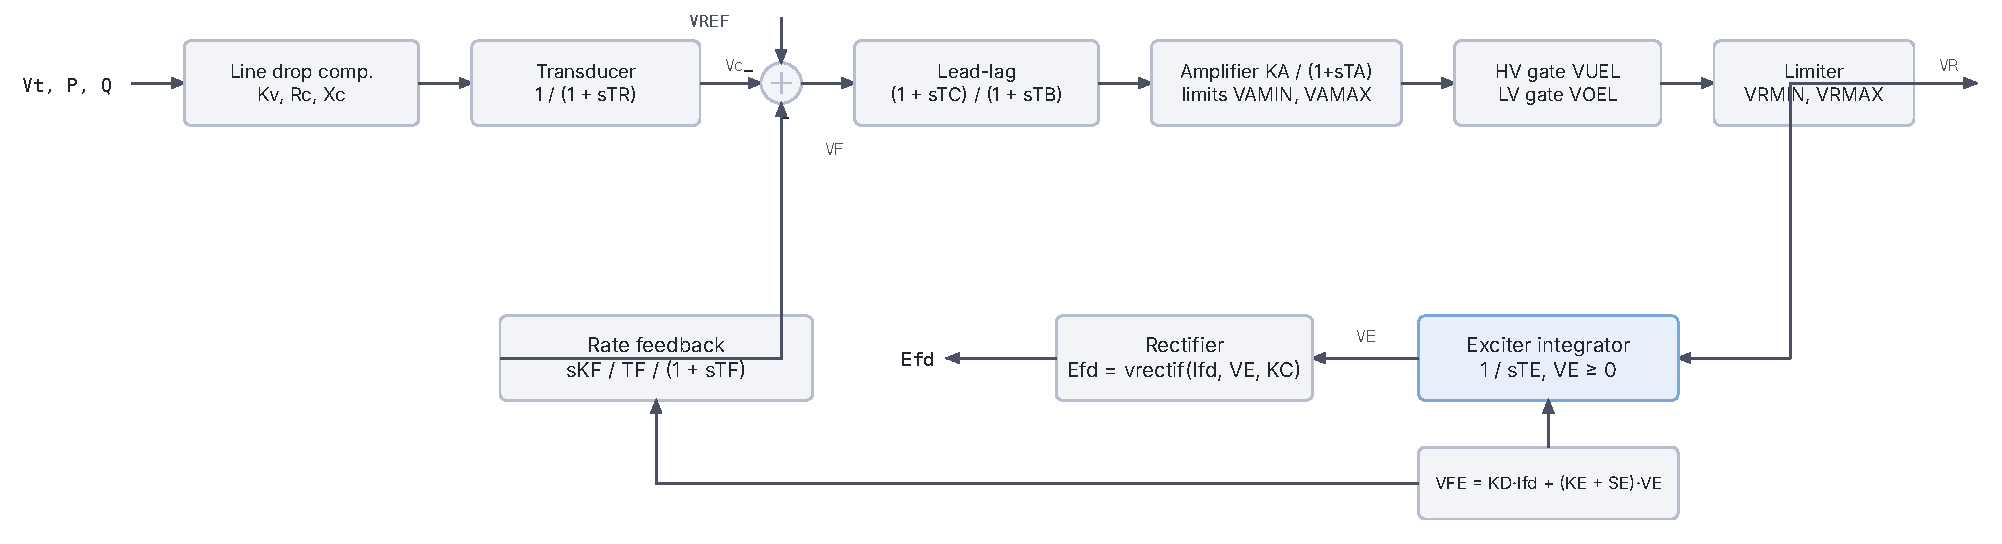
\includegraphics[width=0.98\linewidth]{figures/exc-ac1a-light}
\caption{AC1A block diagram.}
\end{figure}

\subsubsection{Mathematical Description}\label{model-exc-ieee:mathematical-description}

The voltage regulator processes the error signal through a lead-lag network and a limited amplifier:

\[\Delta V = V_{REF} - V_c - V_F - \Delta V_{PSS}\]

\[V_1(s) = \Delta V \cdot \frac{1 + sT_C}{1 + sT_B}\]

\[V_A(s) = V_1 \cdot \frac{K_A}{1 + sT_A}, \quad V_{AMIN} \le V_A \le V_{AMAX}\]

The AC exciter integrator with saturation and demagnetization:

\[V_{FE} = K_D \cdot I_{fd} + \left(K_E + S_E(V_E)\right) V_E\]

\[\dot{V}_E = \frac{1}{T_E}(V_R - V_{FE}), \quad 0 \le V_E\]

\[E_{fd} = V_E \cdot \left(1 - \frac{K_C \cdot I_{fd}}{V_E}\right)\]

The derivative feedback (rate feedback) path:

\[V_F(s) = E_{fd} \cdot \frac{sK_F/T_F}{1 + sT_F}\]

where \(S_E(V_E)\) is the saturation function interpolated from the two-point saturation characteristic \((V_{E1}, SE_1)\) and \((V_{E2}, SE_2)\).

\subsubsection{Signal Flow}\label{model-exc-ieee:signal-flow}

\begin{enumerate}
\def\labelenumi{\arabic{enumi}.}
\tightlist
\item
  \textbf{Line drop compensation} (\texttt{algeq}): \(V_{c1} = vcomp(V_t, P, Q, K_v, R_c, X_c)\)
\item
  \textbf{Voltage measurement filter} (\texttt{tf1p}): \(V_c \leftarrow V_{c1}\) with time constant \(T_R\)
\item
  \textbf{AVR summation} (\texttt{algeq}): \(\Delta V = V_{REF} - V_c - V_F\)
\item
  \textbf{Lead-lag compensator} (\texttt{tf1p1z}): \(V_1 \leftarrow \Delta V\) with \((T_C, T_B)\)
\item
  \textbf{Amplifier with limits} (\texttt{tf1plim}): \(V_2 \leftarrow V_1\) with gain \(K_A\), time constant \(T_A\), limits \([V_{AMIN}, V_{AMAX}]\)
\item
  \textbf{UEL high-value gate} (\texttt{max1v1c}): \(V_3 = \max(V_2, V_{UEL})\)
\item
  \textbf{OEL low-value gate} (\texttt{min1v1c}): \(V_4 = \min(V_3, V_{OEL})\)
\item
  \textbf{Output limiter} (\texttt{lim}): \(V_R = \text{clamp}(V_4, V_{RMIN}, V_{RMAX})\)
\item
  \textbf{Exciter integrator} (\texttt{inlim}): \(V_E \leftarrow (V_R - V_{FE})/T_E\)
\item
  \textbf{Saturation computation} (\texttt{algeq}): \(V_{FE}\) from \(K_D\), \(K_E\), \(S_E(V_E)\)
\item
  \textbf{Rectifier output} (\texttt{algeq}): \(E_{fd} = vrectif(I_{fd}, V_E, K_C)\)
\item
  \textbf{Derivative feedback} (\texttt{tfder1p}): \(V_F \leftarrow V_{FE}\) with gain \(K_F/T_F\), time constant \(T_F\)
\end{enumerate}

\subsubsection{Parameters}\label{model-exc-ieee:parameters}

\begin{small}\begin{longtable}[]{@{}lll@{}}
\toprule\noalign{}
Parameter & Description & Unit/Type \\
\midrule\noalign{}
\endhead
\bottomrule\noalign{}
\endlastfoot
\texttt{Kv} & Voltage compensation gain & pu \\
\texttt{Rc} & Resistance for line drop compensation & pu \\
\texttt{Xc} & Reactance for line drop compensation & pu \\
\texttt{TR} & Voltage transducer time constant & s \\
\texttt{KA} & Voltage regulator gain & pu \\
\texttt{TA} & Voltage regulator time constant & s \\
\texttt{TB} & Lead-lag denominator time constant & s \\
\texttt{TC} & Lead-lag numerator time constant & s \\
\texttt{VAMAX} & Maximum regulator output & pu \\
\texttt{VAMIN} & Minimum regulator output & pu \\
\texttt{KE} & Exciter constant (self-excitation term) & pu \\
\texttt{TE} & Exciter time constant & s \\
\texttt{KF} & Rate feedback gain & pu \\
\texttt{TF} & Rate feedback time constant & s \\
\texttt{VRMAX} & Maximum field voltage & pu \\
\texttt{VRMIN} & Minimum field voltage & pu \\
\texttt{VE1} & Saturation factor voltage point 1 & pu \\
\texttt{SE1} & Saturation factor at \(V_{E1}\) & pu \\
\texttt{VE2} & Saturation factor voltage point 2 & pu \\
\texttt{SE2} & Saturation factor at \(V_{E2}\) & pu \\
\texttt{KC} & Commutation factor (rectifier regulation) & pu \\
\texttt{KD} & Demagnetization factor & pu \\
\texttt{VUEL} & UEL input signal & pu \\
\end{longtable}\end{small}

\subsubsection{Variants}\label{model-exc-ieee:variants}

\begin{small}\begin{longtable}[]{@{}
  >{\raggedright\arraybackslash}p{(\linewidth - 4\tabcolsep) * \real{0.2937}}
  >{\raggedright\arraybackslash}p{(\linewidth - 4\tabcolsep) * \real{0.7063}}
@{}}
\toprule\noalign{}
\begin{minipage}[b]{\linewidth}\raggedright
Model
\end{minipage} & \begin{minipage}[b]{\linewidth}\raggedright
Description
\end{minipage} \\
\midrule\noalign{}
\endhead
\bottomrule\noalign{}
\endlastfoot
\texttt{AC1A} & Base model, IEEE Type AC1A \\
\texttt{AC1A\_MAXEX2} & Adds MAXEX2 field current limiter; VOEL moves to reference summation point (LV gate removed) \\
\texttt{AC1A\_RETRO} & Retrofit variant with internal PSS4B; uses first-order AVR without separate exciter block \\
\texttt{AC1A\_RETRO\_PSS4B} & Retrofit variant with external PSS4B speed input \\
\end{longtable}\end{small}

\subsubsection{Usage Example}\label{model-exc-ieee:usage-example}

\begin{Verbatim}
SYNC_MACH g1  g1  1. 1.  0.  0.   800. 760. 3. 0. 0.95
                    XT   0.15  1.1  0.25  0.2  0.7  *  0.2  0.1  6.0257  0.  5.00  0.05  *  0.1
              EXC AC1A   0. 0. 0. 0.02 200.0 0.02 10.0 1.0 7.32 -7.32 1.0 1.0 0.03 1.0 6.03 -5.43 4.18 0.1 3.14 0.033 0.2 0.38 99999
              TOR CONSTANT ;
\end{Verbatim}

\begin{center}\rule{0.5\linewidth}{0.5pt}\end{center}

\subsection{AC4A}\label{model-exc-ieee:ac4a}

The AC4A is a simplified static representation of an AC exciter system with an inner-loop voltage-dependent output limit. It corresponds to IEEE Std 421.5-2016 Type AC4A. The upper output limit is a function of field current: \(V_{RMAX,eff} = V_{RMAX} - K_C \cdot I_{fd}\).

\begin{figure}[htbp]
\centering
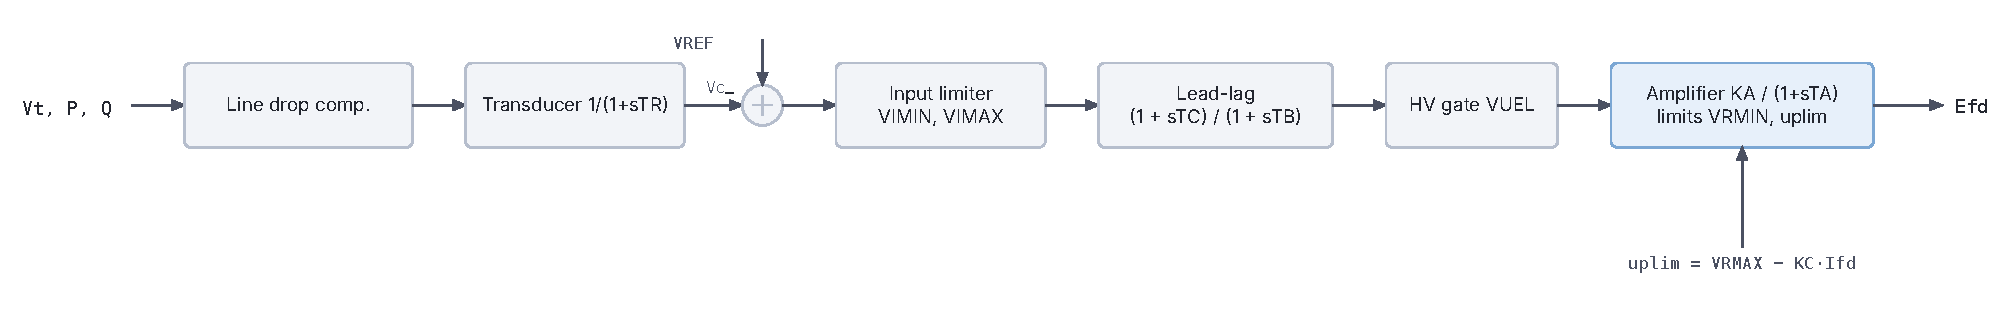
\includegraphics[width=0.98\linewidth]{figures/exc-ac4a-light}
\caption{AC4A block diagram.}
\end{figure}

\subsubsection{Mathematical Description}\label{model-exc-ieee:mathematical-description-1}

\[\Delta V = V_{REF} - V_c\]

\[V_I = \text{clamp}(\Delta V, V_{IMIN}, V_{IMAX})\]

\[V_1(s) = V_I \cdot \frac{1 + sT_C}{1 + sT_B}\]

\[E_{fd}(s) = V_1 \cdot \frac{K_A}{1 + sT_A}, \quad V_{RMIN} \le E_{fd} \le V_{RMAX} - K_C \cdot I_{fd}\]

The variable upper limit is updated algebraically at each time step, making AC4A a time-varying limited integrator system.

\subsubsection{Signal Flow}\label{model-exc-ieee:signal-flow-1}

\begin{enumerate}
\def\labelenumi{\arabic{enumi}.}
\tightlist
\item
  \textbf{Line drop compensation} (\texttt{algeq}): \(V_{c1}\) from terminal measurements
\item
  \textbf{Voltage measurement filter} (\texttt{tf1p}): \(V_c\) with \(T_R\)
\item
  \textbf{AVR summation} (\texttt{algeq}): \(\Delta V = V_{REF} - V_c\)
\item
  \textbf{Input limiter} (\texttt{lim}): \(V_I = \text{clamp}(\Delta V, V_{IMIN}, V_{IMAX})\)
\item
  \textbf{Lead-lag} (\texttt{tf1p1z}): \(V_1 \leftarrow V_I\) with \((T_C, T_B)\)
\item
  \textbf{UEL high-value gate} (\texttt{max1v1c}): \(V_2 = \max(V_1, V_{UEL})\)
\item
  \textbf{Variable upper limit} (\texttt{algeq}): \(uplim = V_{RMAX} - K_C \cdot I_{fd}\)
\item
  \textbf{Variable-limit amplifier} (\texttt{tf1pvlim}): \(E_{fd} \leftarrow V_2\) with \(K_A\), \(T_A\), limits \([V_{RMIN}, uplim]\)
\end{enumerate}

\subsubsection{Parameters}\label{model-exc-ieee:parameters-1}

\begin{small}\begin{longtable}[]{@{}lll@{}}
\toprule\noalign{}
Parameter & Description & Unit/Type \\
\midrule\noalign{}
\endhead
\bottomrule\noalign{}
\endlastfoot
\texttt{Kv} & Voltage compensation gain & pu \\
\texttt{Rc} & Line drop compensation resistance & pu \\
\texttt{Xc} & Line drop compensation reactance & pu \\
\texttt{TR} & Measurement filter time constant & s \\
\texttt{VIMAX} & Maximum input error signal & pu \\
\texttt{VIMIN} & Minimum input error signal & pu \\
\texttt{TC} & Lead numerator time constant & s \\
\texttt{TB} & Lag denominator time constant & s \\
\texttt{VUEL} & UEL signal value & pu \\
\texttt{KA} & Regulator gain & pu \\
\texttt{TA} & Regulator time constant & s \\
\texttt{VRMAX} & Maximum output (at zero field current) & pu \\
\texttt{VRMIN} & Minimum output & pu \\
\texttt{KC} & Field current derating factor & pu \\
\end{longtable}\end{small}

\subsubsection{Variants}\label{model-exc-ieee:variants-1}

\begin{small}\begin{longtable}[]{@{}ll@{}}
\toprule\noalign{}
Model & Description \\
\midrule\noalign{}
\endhead
\bottomrule\noalign{}
\endlastfoot
\texttt{AC4A} & Base model, IEEE Type AC4A, no PSS or OEL \\
\end{longtable}\end{small}

\subsubsection{Usage Example}\label{model-exc-ieee:usage-example-1}

\begin{Verbatim}
SYNC_MACH g1  g1  1. 1.  0.  0.   800. 760. 3. 0. 0.95
                    XT   0.15  1.1  0.25  0.2  0.7  *  0.2  0.1  6.0257  0.  5.00  0.05  *  0.1
              EXC AC4A   0. 0. 0. 0.02 8.0 -8.0 1.0 10.0 0.0 200.0 0.015 4.44 -4.44 0.0
              TOR CONSTANT ;
\end{Verbatim}

\begin{center}\rule{0.5\linewidth}{0.5pt}\end{center}

\subsection{AC8B}\label{model-exc-ieee:ac8b}

The AC8B is a rotating AC exciter with a PID voltage regulator (rather than the proportional-integral amplifier of earlier types). It corresponds to IEEE Std 421.5-2016 Type AC8B. The PID structure, proportional gain \(K_{PR}\), integral gain \(K_{IR}\), and derivative gain \(K_{DR}\), provides improved transient response compared to Type AC1A.

\begin{figure}[htbp]
\centering
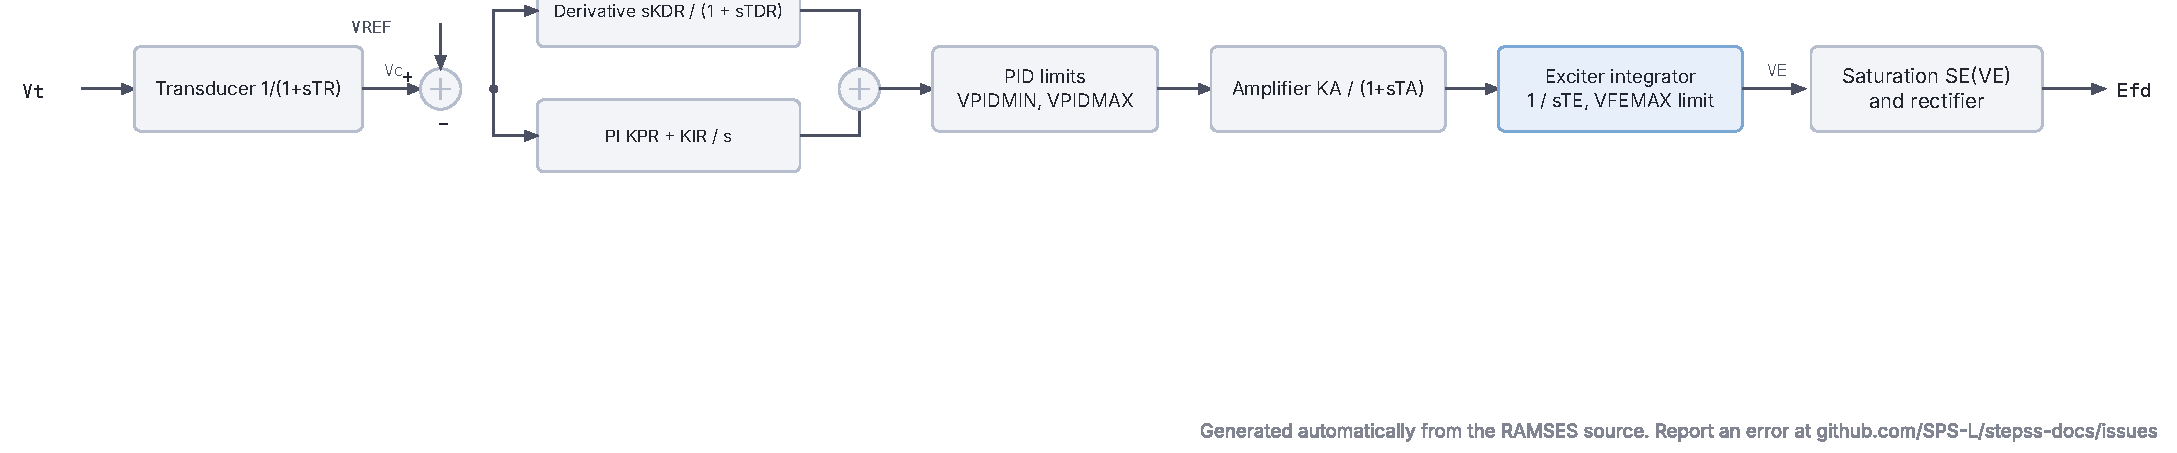
\includegraphics[width=0.98\linewidth]{figures/exc-ac8b-light}
\caption{AC8B block diagram.}
\end{figure}

\subsubsection{Mathematical Description}\label{model-exc-ieee:mathematical-description-2}

The PID voltage regulator:

\[\Delta V = V_c - V_{REF}\]

\[V_{PID}(s) = K_{PR} \cdot \Delta V + \frac{K_{IR}}{s} \cdot \Delta V + \frac{sK_{DR}/T_{DR}}{1 + sT_{DR}} \cdot \Delta V\]

\[V_R(s) = V_{PID} \cdot \frac{K_A}{1 + sT_A}, \quad V_{RMIN} \le V_R \le V_{RMAX}\]

The AC exciter with variable limits based on maximum field excitation voltage \(V_{FEMAX}\):

\[V_{FE} = K_D \cdot I_{fd} + \left(K_E + S_E(V_E)\right) V_E\]

\[\dot{V}_E = \frac{1}{T_E}(V_R - V_{FE}), \quad V_{EMIN} \le V_E \le \frac{V_{FEMAX} - K_D I_{fd}}{K_E + S_E(V_E)}\]

\subsubsection{Signal Flow}\label{model-exc-ieee:signal-flow-2}

\begin{enumerate}
\def\labelenumi{\arabic{enumi}.}
\tightlist
\item
  \textbf{Voltage measurement} (\texttt{tf1p}): \(V_c\) with \(T_R\)
\item
  \textbf{Error signal} (\texttt{algeq}): \(\Delta V = V_c - V_{REF}\)
\item
  \textbf{PID derivative part} (\texttt{tfder1p}): \(x_{der} \leftarrow \Delta V\) with gain \(K_{DR}/T_{DR}\)
\item
  \textbf{PID proportional-integral} (\texttt{pictl}): \(x_{propint} \leftarrow \Delta V\) with \(K_{IR}\), \(K_{PR}\)
\item
  \textbf{PID sum} (\texttt{algeq}): \(x_{pid} = x_{propint} + x_{der}\), limited to \([V_{PIDMIN}, V_{PIDMAX}]\)
\item
  \textbf{Amplifier} (\texttt{tf1plim}): \(V_R \leftarrow x_{pid}\) with \(K_A\), \(T_A\)
\item
  \textbf{Exciter integrator} (\texttt{invlim}): \(V_E\) with variable limits from \(V_{FEMAX}\)
\item
  \textbf{Saturation and rectification} (\texttt{algeq}): \(V_{FE}\), \(E_{fd}\)
\end{enumerate}

\subsubsection{Parameters}\label{model-exc-ieee:parameters-2}

\begin{small}\begin{longtable}[]{@{}lll@{}}
\toprule\noalign{}
Parameter & Description & Unit/Type \\
\midrule\noalign{}
\endhead
\bottomrule\noalign{}
\endlastfoot
\texttt{Kv} & Voltage compensation gain & pu \\
\texttt{Rc} & Line drop resistance & pu \\
\texttt{Xc} & Line drop reactance & pu \\
\texttt{TR} & Measurement time constant & s \\
\texttt{KPR} & PID proportional gain & pu \\
\texttt{KIR} & PID integral gain & pu/s \\
\texttt{KDR} & PID derivative gain & pu\ensuremath{\cdot}s \\
\texttt{TDR} & PID derivative filter time constant & s \\
\texttt{VPIDMAX} & PID output upper limit & pu \\
\texttt{VPIDMIN} & PID output lower limit & pu \\
\texttt{KA} & Amplifier gain & pu \\
\texttt{TA} & Amplifier time constant & s \\
\texttt{VRMAX} & Maximum regulator output & pu \\
\texttt{VRMIN} & Minimum regulator output & pu \\
\texttt{KC} & Rectifier commutation factor & pu \\
\texttt{KD} & Demagnetization factor & pu \\
\texttt{KE} & Exciter self-excitation constant & pu \\
\texttt{TE} & Exciter time constant & s \\
\texttt{VFEMAX} & Maximum field excitation voltage & pu \\
\texttt{VEMIN} & Minimum exciter output & pu \\
\texttt{VE1} & Saturation voltage point 1 & pu \\
\texttt{SE1} & Saturation factor at \(V_{E1}\) & pu \\
\texttt{VE2} & Saturation voltage point 2 & pu \\
\texttt{SE2} & Saturation factor at \(V_{E2}\) & pu \\
\end{longtable}\end{small}

\subsubsection{Variants}\label{model-exc-ieee:variants-2}

\begin{small}\begin{longtable}[]{@{}
  >{\raggedright\arraybackslash}p{(\linewidth - 4\tabcolsep) * \real{0.3097}}
  >{\raggedright\arraybackslash}p{(\linewidth - 4\tabcolsep) * \real{0.6903}}
@{}}
\toprule\noalign{}
\begin{minipage}[b]{\linewidth}\raggedright
Model
\end{minipage} & \begin{minipage}[b]{\linewidth}\raggedright
Description
\end{minipage} \\
\midrule\noalign{}
\endhead
\bottomrule\noalign{}
\endlastfoot
\texttt{AC8B} & Base model, IEEE Type AC8B \\
\texttt{AC8B\_PSS3B\_lim} & Adds PSS3B dual-input stabilizer and integral OEL + SCL (stator current limiter) \\
\texttt{AC8B\_lim} & Adds integral OEL and SCL without PSS \\
\end{longtable}\end{small}

\subsubsection{Usage Example}\label{model-exc-ieee:usage-example-2}

\begin{Verbatim}
SYNC_MACH g1  g1  1. 1.  0.  0.   800. 760. 3. 0. 0.95
                    XT   0.15  1.1  0.25  0.2  0.7  *  0.2  0.1  6.0257  0.  5.00  0.05  *  0.1
              EXC AC8B   0. 0. 0. 0.02 1.0 5.0 0.1 0.1 8.0 -8.0 1.0 0.1 6.5 -6.5 0.2 1.0 1.0 0.5 6.5 0.0 4.0 0.3 3.0 0.33
              TOR CONSTANT ;
\end{Verbatim}

\begin{center}\rule{0.5\linewidth}{0.5pt}\end{center}

\section{DC Exciter Models}\label{model-exc-ieee:dc-exciter-models}

\subsection{DC3A}\label{model-exc-ieee:dc3a}

The DC3A represents a non-continuously acting (rheostat-type) DC excitation system. It corresponds to IEEE Std 421.5-2016 Type DC3A. Rather than a proportional amplifier, it uses a three-position switch (VRMIN / VRH / VRMAX) driven by an integrator that holds the rheostat position \(V_{RH}\). The switch position is determined by whether the error signal \(V_{ERR}\) falls inside or outside a deadband \(\pm K_V\).

\begin{figure}[htbp]
\centering
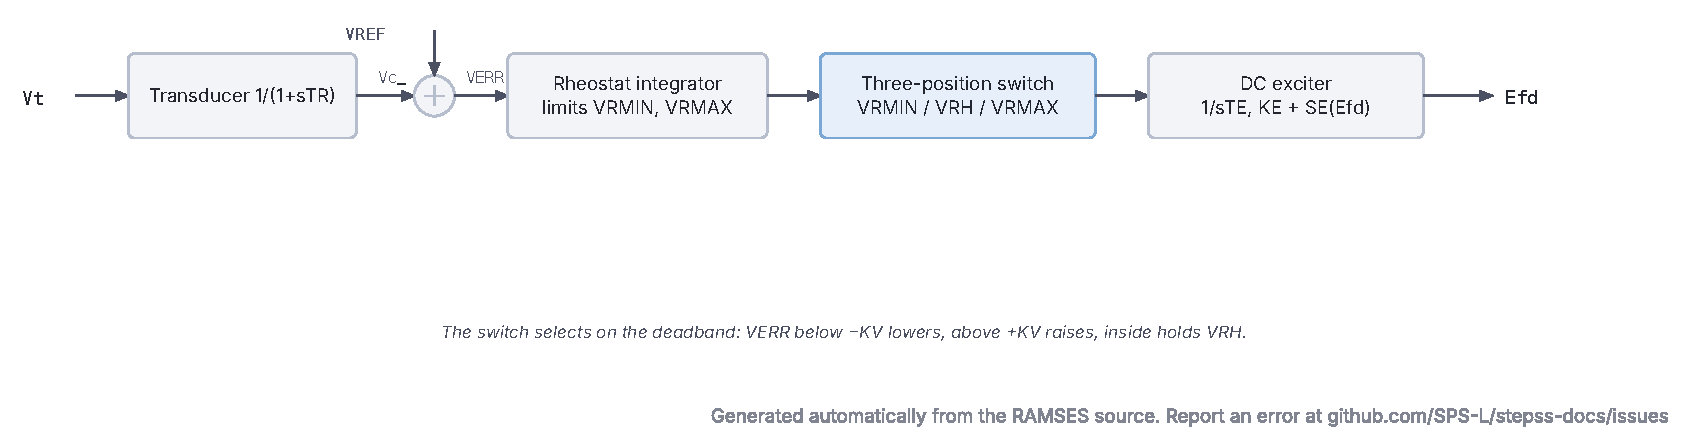
\includegraphics[width=0.98\linewidth]{figures/exc-dc3a-light}
\caption{DC3A block diagram.}
\end{figure}

\subsubsection{Mathematical Description}\label{model-exc-ieee:mathematical-description-3}

\[V_{ERR} = V_{REF} - V_c\]

The rheostat integrator:

\[\dot{V}_{RH} = \frac{K_V \cdot T_{RH}}{V_{RMAX} - V_{RMIN}} \cdot \text{clamp}(V_{ERR}, -K_V, K_V), \quad V_{RMIN} \le V_{RH} \le V_{RMAX}\]

The three-position switch:

\[V_R = \begin{cases} V_{RMIN} & V_{ERR} < -K_V \\ V_{RH} & |V_{ERR}| \le K_V \\ V_{RMAX} & V_{ERR} > K_V \end{cases}\]

The DC exciter with saturation:

\[\dot{E}_{fd} = \frac{1}{T_E}\left[V_R - \left(K_E + S_E(E_{fd})\right) E_{fd}\right]\]

\subsubsection{Parameters}\label{model-exc-ieee:parameters-3}

\begin{small}\begin{longtable}[]{@{}lll@{}}
\toprule\noalign{}
Parameter & Description & Unit/Type \\
\midrule\noalign{}
\endhead
\bottomrule\noalign{}
\endlastfoot
\texttt{Kvcomp} & Voltage compensation gain & pu \\
\texttt{Rc} & Line drop resistance & pu \\
\texttt{Xc} & Line drop reactance & pu \\
\texttt{TR} & Measurement time constant & s \\
\texttt{TRH} & Rheostat traversal time & s \\
\texttt{KV} & Sensitivity of non-continuously acting controller & pu \\
\texttt{VRMAX} & Maximum field voltage & pu \\
\texttt{VRMIN} & Minimum field voltage & pu \\
\texttt{TE} & Exciter time constant & s \\
\texttt{KE} & Exciter self-excitation constant & pu \\
\texttt{E1} & Saturation voltage point 1 & pu \\
\texttt{SE1} & Saturation factor at \(E_1\) & pu \\
\texttt{E2} & Saturation voltage point 2 & pu \\
\texttt{SE2} & Saturation factor at \(E_2\) & pu \\
\end{longtable}\end{small}

\subsubsection{Variants}\label{model-exc-ieee:variants-3}

\begin{small}\begin{longtable}[]{@{}
  >{\raggedright\arraybackslash}p{(\linewidth - 4\tabcolsep) * \real{0.2489}}
  >{\raggedright\arraybackslash}p{(\linewidth - 4\tabcolsep) * \real{0.7511}}
@{}}
\toprule\noalign{}
\begin{minipage}[b]{\linewidth}\raggedright
Model
\end{minipage} & \begin{minipage}[b]{\linewidth}\raggedright
Description
\end{minipage} \\
\midrule\noalign{}
\endhead
\bottomrule\noalign{}
\endlastfoot
\texttt{DC3A} & Base model, IEEE Type DC3A, non-continuously acting rheostat controller \\
\end{longtable}\end{small}

\subsubsection{Usage Example}\label{model-exc-ieee:usage-example-3}

\begin{Verbatim}
SYNC_MACH g1  g1  1. 1.  0.  0.   800. 760. 3. 0. 0.95
                    XT   0.15  1.1  0.25  0.2  0.7  *  0.2  0.1  6.0257  0.  5.00  0.05  *  0.1
              EXC DC3A   0. 0. 0. 0.0 1.0 1.0 1.0 -1.0 0.8 1.0 3.1 0.33 2.3 0.1
              TOR CONSTANT ;
\end{Verbatim}

\begin{center}\rule{0.5\linewidth}{0.5pt}\end{center}

\section{ST (Static) Exciter Models}\label{model-exc-ieee:st-static-exciter-models}

\subsection{ST1A}\label{model-exc-ieee:st1a}

The ST1A is a static (thyristor) excitation system with two cascaded lead-lag networks in the voltage regulator path and an inner field current limiter (KLR/ILR). It corresponds to IEEE Std 421.5-2016 Type ST1A. The output limits are proportional to terminal voltage \(V_t\), and field current derating applies through \(K_C\): \(uplim = V_t \cdot V_{RMAX} - K_C \cdot I_{fd}\).

\begin{figure}[htbp]
\centering
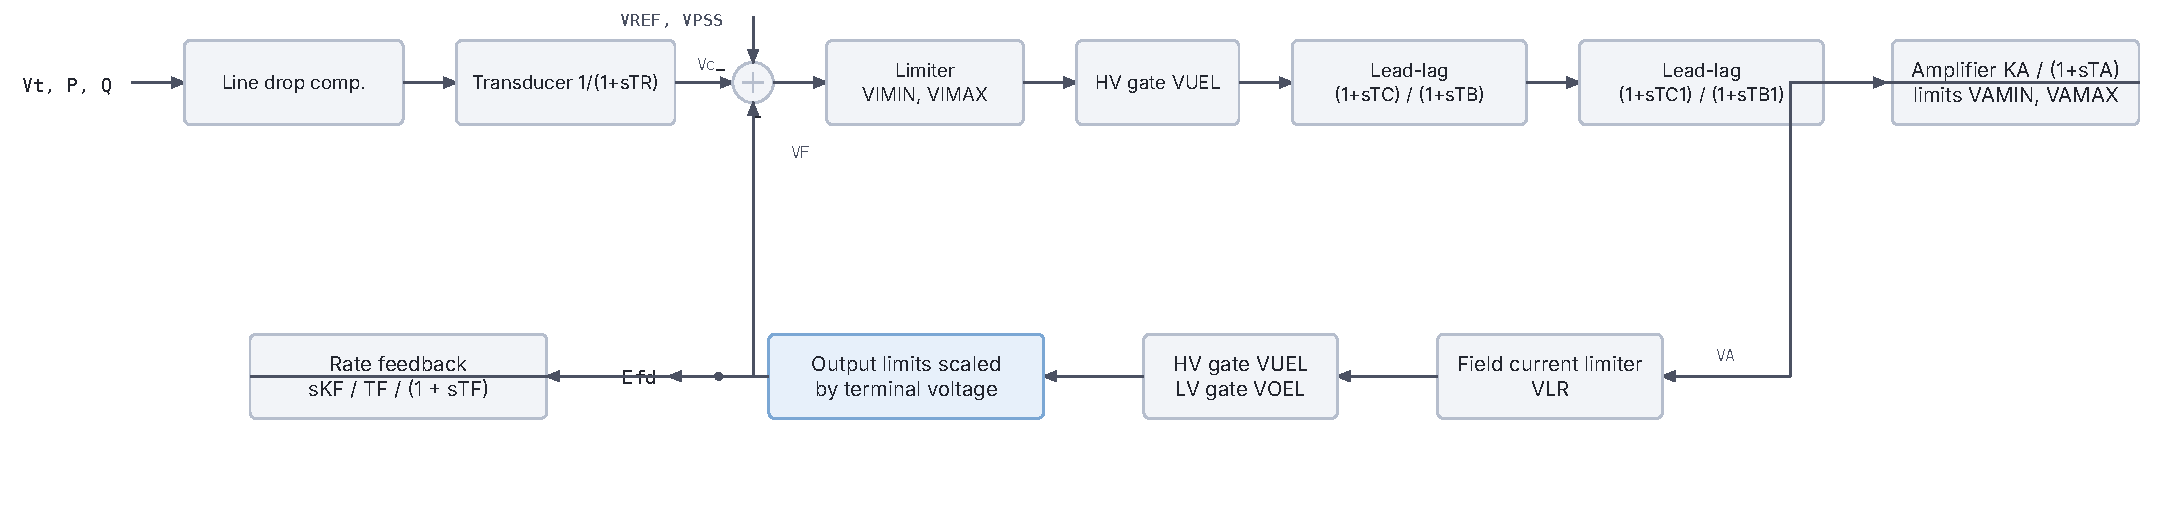
\includegraphics[width=0.98\linewidth]{figures/exc-st1a-light}
\caption{ST1A block diagram.}
\end{figure}

\subsubsection{Mathematical Description}\label{model-exc-ieee:mathematical-description-4}

The voltage regulator with dual lead-lag and instantaneous field current limiting:

\[\Delta V = V_{REF} - V_c + V_{PSS} + V_{UEL,path} + V_F\]

\[V_1 = \text{clamp}(\Delta V, V_{IMIN}, V_{IMAX})\]

\[V_2(s) = V_1 \cdot \frac{1 + sT_C}{1 + sT_B}\]

\[V_3(s) = V_2 \cdot \frac{1 + sT_{C1}}{1 + sT_{B1}}\]

\[V_A(s) = V_3 \cdot \frac{K_A}{1 + sT_A}, \quad V_{AMIN} \le V_A \le V_{AMAX}\]

Instantaneous field current limiter:

\[V_{LR} = K_{LR}(I_{fd} - I_{LR})\]

\[V_5 = V_A - \max(V_{LR}, 0)\]

Final output with terminal-voltage-dependent limits:

\[E_{fd} = \text{clamp}(V_5, V_t \cdot V_{RMIN}, V_t \cdot V_{RMAX} - K_C \cdot I_{fd})\]

Derivative feedback:

\[V_F(s) = E_{fd} \cdot \frac{sK_F/T_F}{1 + sT_F}\]

\subsubsection{Signal Flow}\label{model-exc-ieee:signal-flow-3}

\begin{enumerate}
\def\labelenumi{\arabic{enumi}.}
\tightlist
\item
  \textbf{Line drop} (\texttt{algeq}): \(V_{c1}\)
\item
  \textbf{Measurement filter} (\texttt{tf1p}): \(V_c\) with \(T_R\)
\item
  \textbf{AVR summation} (\texttt{algeq}): \(\Delta V\), including UEL (mode 1), PSS, and VF
\item
  \textbf{Error limiter} (\texttt{lim}): \(V_1 \in [V_{IMIN}, V_{IMAX}]\)
\item
  \textbf{UEL gate (mode 2)} (\texttt{max1v1c}): HV gate \(V_2\)
\item
  \textbf{First lead-lag} (\texttt{tf1p1z}): \(V_3\) with \((T_C, T_B)\)
\item
  \textbf{Second lead-lag} (\texttt{tf1p1z}): \(V_4\) with \((T_{C1}, T_{B1})\)
\item
  \textbf{Amplifier} (\texttt{tf1plim}): \(V_A\) with \(K_A\), \(T_A\), \([V_{AMIN}, V_{AMAX}]\)
\item
  \textbf{Field current limiter} (\texttt{algeq}, \texttt{lim}): \(V_{LR}\), \(V_{LRlim}\)
\item
  \textbf{Limiter subtraction} (\texttt{algeq}): \(V_5 = V_A - V_{LRlim}\)
\item
  \textbf{UEL gate (mode 3)} (\texttt{max1v1c}): \(V_6\)
\item
  \textbf{OEL gate} (\texttt{min2v}): \(V_7 = \min(V_6, V_{OEL})\)
\item
  \textbf{Variable-limit output} (\texttt{limvb}): \(E_{fd}\) with terminal-voltage-scaled limits
\item
  \textbf{Derivative feedback} (\texttt{tfder1p}): \(V_F\)
\end{enumerate}

\subsubsection{Parameters}\label{model-exc-ieee:parameters-4}

\begin{small}\begin{longtable}[]{@{}
  >{\raggedright\arraybackslash}p{(\linewidth - 6\tabcolsep) * \real{0.2133}}
  >{\raggedright\arraybackslash}p{(\linewidth - 6\tabcolsep) * \real{0.5939}}
  >{\raggedright\arraybackslash}p{(\linewidth - 6\tabcolsep) * \real{0.1928}}
@{}}
\toprule\noalign{}
\begin{minipage}[b]{\linewidth}\raggedright
Parameter
\end{minipage} & \begin{minipage}[b]{\linewidth}\raggedright
Description
\end{minipage} & \begin{minipage}[b]{\linewidth}\raggedright
Unit/Type
\end{minipage} \\
\midrule\noalign{}
\endhead
\bottomrule\noalign{}
\endlastfoot
\texttt{Kv} & Voltage compensation gain & pu \\
\texttt{Rc} & Line drop resistance & pu \\
\texttt{Xc} & Line drop reactance & pu \\
\texttt{TR} & Measurement filter time constant & s \\
\texttt{UEL} & UEL connection mode (1=summation, 2=HV gate after V1, 3=HV gate after VA) & integer \\
\texttt{VIMIN} & Input error lower limit & pu \\
\texttt{VIMAX} & Input error upper limit & pu \\
\texttt{VUEL} & UEL signal value & pu \\
\texttt{TC} & First lead-lag numerator & s \\
\texttt{TB} & First lead-lag denominator & s \\
\texttt{TC1} & Second lead-lag numerator & s \\
\texttt{TB1} & Second lead-lag denominator & s \\
\texttt{KA} & Regulator gain & pu \\
\texttt{TA} & Regulator time constant & s \\
\texttt{VAMIN} & Regulator lower limit & pu \\
\texttt{VAMAX} & Regulator upper limit & pu \\
\texttt{VRMIN} & Output lower limit scaling factor & pu \\
\texttt{VRMAX} & Output upper limit scaling factor & pu \\
\texttt{KC} & Field current derating factor & pu \\
\texttt{KF} & Rate feedback gain & pu \\
\texttt{TF} & Rate feedback time constant & s \\
\texttt{KLR} & Field current limiter gain & pu \\
\texttt{ILR} & Field current limiter reference & pu \\
\end{longtable}\end{small}

\subsubsection{Variants}\label{model-exc-ieee:variants-4}

\begin{small}\begin{longtable}[]{@{}
  >{\raggedright\arraybackslash}p{(\linewidth - 4\tabcolsep) * \real{0.3489}}
  >{\raggedright\arraybackslash}p{(\linewidth - 4\tabcolsep) * \real{0.6511}}
@{}}
\toprule\noalign{}
\begin{minipage}[b]{\linewidth}\raggedright
Model
\end{minipage} & \begin{minipage}[b]{\linewidth}\raggedright
Description
\end{minipage} \\
\midrule\noalign{}
\endhead
\bottomrule\noalign{}
\endlastfoot
\texttt{ST1A} & Base model, IEEE Type ST1A \\
\texttt{ST1A\_IEEEST} & Adds IEEEST single-input PSS (speed or power input, selectable) \\
\texttt{ST1A\_IEEEST\_MAXEX2} & Adds IEEEST PSS + MAXEX2 field current limiter \\
\texttt{ST1A\_PSS2B} & Adds PSS2B dual-input stabilizer \\
\texttt{ST1A\_PSS2B\_MAXEX2} & Adds PSS2B + MAXEX2 \\
\texttt{ST1A\_PSS3B} & Adds PSS3B two-channel second-order filter stabilizer \\
\texttt{ST1A\_PSS4B} & Adds PSS4B three-band stabilizer \\
\texttt{ST1A\_PSS4B\_MAXEX2} & Adds PSS4B + MAXEX2 \\
\texttt{ST1A\_lim} & Integral OEL + stator current limiter (SCL), simplified structure without Kv/Rc/Xc \\
\end{longtable}\end{small}

\subsubsection{Usage Example}\label{model-exc-ieee:usage-example-4}

\begin{Verbatim}
SYNC_MACH g1  g1  1. 1.  0.  0.   800. 760. 3. 0. 0.95
                    XT   0.15  1.1  0.25  0.2  0.7  *  0.2  0.1  6.0257  0.  5.00  0.05  *  0.1
              EXC ST1A   0. 0. 0. 0.02 1 -0.87 0.87 0.0 1.0 10.0 0.0 1.0 200.0 0.001 7.8 -6.7 0.038 0.0 999.0 0.0 99.0 0.0 0.0
              TOR CONSTANT ;
\end{Verbatim}

\begin{center}\rule{0.5\linewidth}{0.5pt}\end{center}

\subsection{ST2A (via EXPIC1)}\label{model-exc-ieee:st2a-via-expic1}

The EXPIC1 model implements a static exciter with an AC rotating bus-fed rectifier and an integrating (PI-type) amplifier path: \(K_A(1 + sT_A)/s\). The output \(V_B\) is proportional to the AC voltage phasor magnitude, creating a bus-fed topology analogous to IEEE Type ST2A. When \(K_P = K_I = 0\), the rectifier gain is unity.

\begin{figure}[htbp]
\centering
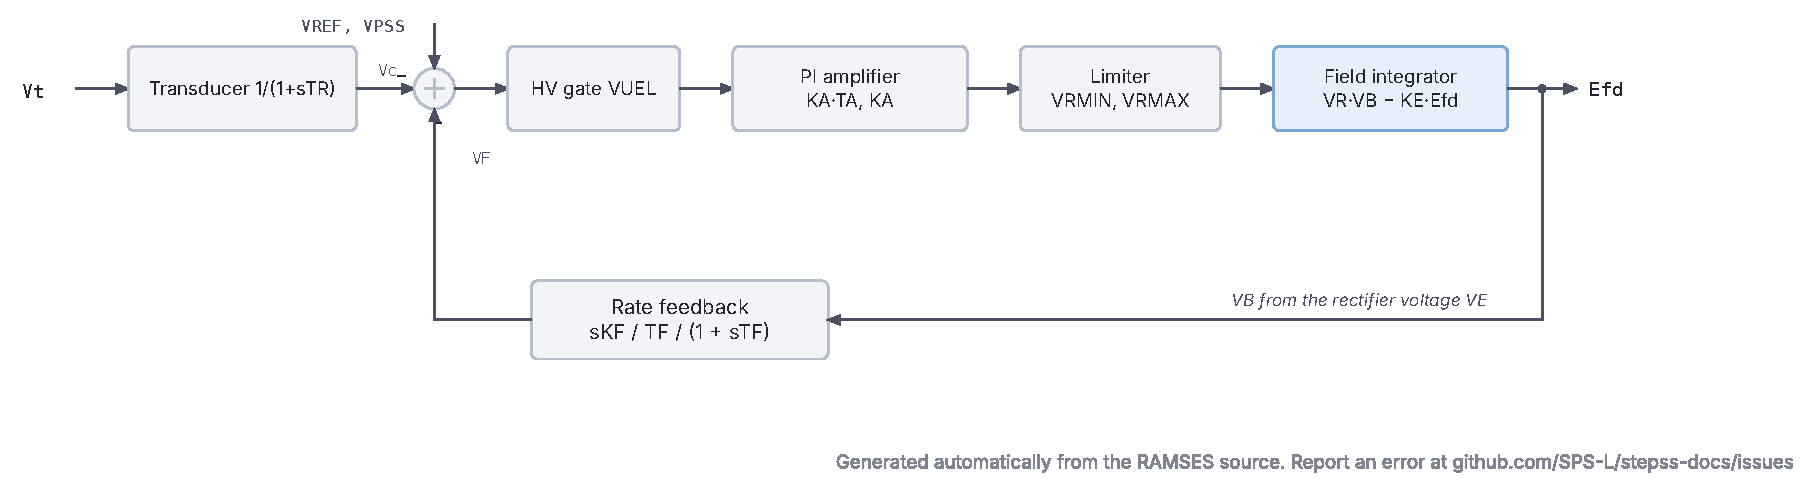
\includegraphics[width=0.98\linewidth]{figures/exc-st2a-light}
\caption{ST2A block diagram.}
\end{figure}

\subsubsection{Mathematical Description}\label{model-exc-ieee:mathematical-description-5}

The AC exciter voltage and rectifier:

\[V_E = |K_P V_t + jK_I V_t|, \quad V_B = V_E \cdot \left(1 - \frac{K_C I_{fd}}{V_E}\right)^+\]

The integrating amplifier:

\[G_{amp}(s) = K_A \cdot \frac{1 + sT_A}{s}\]

The field voltage integrator:

\[\dot{E}_{fd} = \frac{1}{T_E}\left[V_R \cdot V_B - K_E \cdot E_{fd}\right], \quad E_{FDMIN} \le E_{fd} \le E_{FDMAX}\]

\subsubsection{Signal Flow}\label{model-exc-ieee:signal-flow-4}

\begin{enumerate}
\def\labelenumi{\arabic{enumi}.}
\tightlist
\item
  \textbf{Voltage measurement} (\texttt{tf1p}): \(V_c\) with \(T_R\)
\item
  \textbf{Summation} (\texttt{algeq}): \(\Delta V = V_{REF} - V_c - V_F - \Delta V_{PSS}\)
\item
  \textbf{UEL gate} (\texttt{max1v1c}): clamped to \(V_{UEL}\)
\item
  \textbf{PI amplifier} (\texttt{pictl}): \(V_A\) with \(K_{gain} = K_A \cdot T_A\) and \(K_A\)
\item
  \textbf{Output limiter} (\texttt{lim}): \(V_R \in [V_{RMIN}, V_{RMAX}]\)
\item
  \textbf{Rectifier voltage} (\texttt{algeq}): \(V_E\), \(V_B\)
\item
  \textbf{Field integrator} (\texttt{inlim}): \(E_{fd}\) from \(V_R \cdot V_B - K_E \cdot E_{fd}\)
\item
  \textbf{Derivative feedback} (\texttt{tfder1p}): \(V_F\)
\end{enumerate}

\subsubsection{Parameters}\label{model-exc-ieee:parameters-5}

\begin{small}\begin{longtable}[]{@{}lll@{}}
\toprule\noalign{}
Parameter & Description & Unit/Type \\
\midrule\noalign{}
\endhead
\bottomrule\noalign{}
\endlastfoot
\texttt{Kvcomp} & Voltage compensation gain & pu \\
\texttt{Rc} & Line drop resistance & pu \\
\texttt{Xc} & Line drop reactance & pu \\
\texttt{TR} & Measurement time constant & s \\
\texttt{VUEL} & UEL signal & pu \\
\texttt{KA} & Amplifier gain & pu \\
\texttt{TA} & Amplifier time constant & s \\
\texttt{VRMAX} & Maximum regulator output & pu \\
\texttt{VRMIN} & Minimum regulator output & pu \\
\texttt{KF} & Rate feedback gain & pu \\
\texttt{TF} & Rate feedback time constant & s \\
\texttt{KE} & Exciter self-excitation constant & pu \\
\texttt{EFDMAX} & Maximum field voltage & pu \\
\texttt{EFDMIN} & Minimum field voltage & pu \\
\texttt{TE} & Field integrator time constant & s \\
\texttt{KP} & AC source voltage proportional factor & pu \\
\texttt{KI} & AC source voltage quadrature factor & pu \\
\texttt{KC} & Commutation voltage drop factor & pu \\
\end{longtable}\end{small}

\subsubsection{Variants}\label{model-exc-ieee:variants-5}

\begin{small}\begin{longtable}[]{@{}ll@{}}
\toprule\noalign{}
Model & Description \\
\midrule\noalign{}
\endhead
\bottomrule\noalign{}
\endlastfoot
\texttt{EXPIC1} & Base bus-fed static exciter \\
\texttt{EXPIC1\_PSS2B} & Adds PSS2B dual-input stabilizer \\
\texttt{EXPIC1\_PSS2B\_MAXEX2} & Adds PSS2B + MAXEX2 field current limiter \\
\end{longtable}\end{small}

\subsubsection{Usage Example}\label{model-exc-ieee:usage-example-5}

\begin{Verbatim}
SYNC_MACH g1  g1  1. 1.  0.  0.   800. 760. 3. 0. 0.95
                    XT   0.15  1.1  0.25  0.2  0.7  *  0.2  0.1  6.0257  0.  5.00  0.05  *  0.1
              EXC EXPIC1   0. 0. 0. 0.02 0.0 200.0 0.02 99.0 -99.0 0.0 1.0 1.0 8.0 -8.0 0.5 0.0 1.0 0.0
              TOR CONSTANT ;
\end{Verbatim}

\begin{center}\rule{0.5\linewidth}{0.5pt}\end{center}

\section{Other IEEE Models}\label{model-exc-ieee:other-ieee-models}

\subsection{IEEET5}\label{model-exc-ieee:ieeet5}

The IEEET5 (also referenced as DC5A in some conventions) is a non-continuously acting exciter similar to DC3A but uses an inner limiter block \texttt{lim\_civ} that gates the integrator holding signal within a deadband \(\pm K_V\). This creates the three-state (hold/raise/lower) behavior of rheostatic controllers.

\begin{figure}[htbp]
\centering
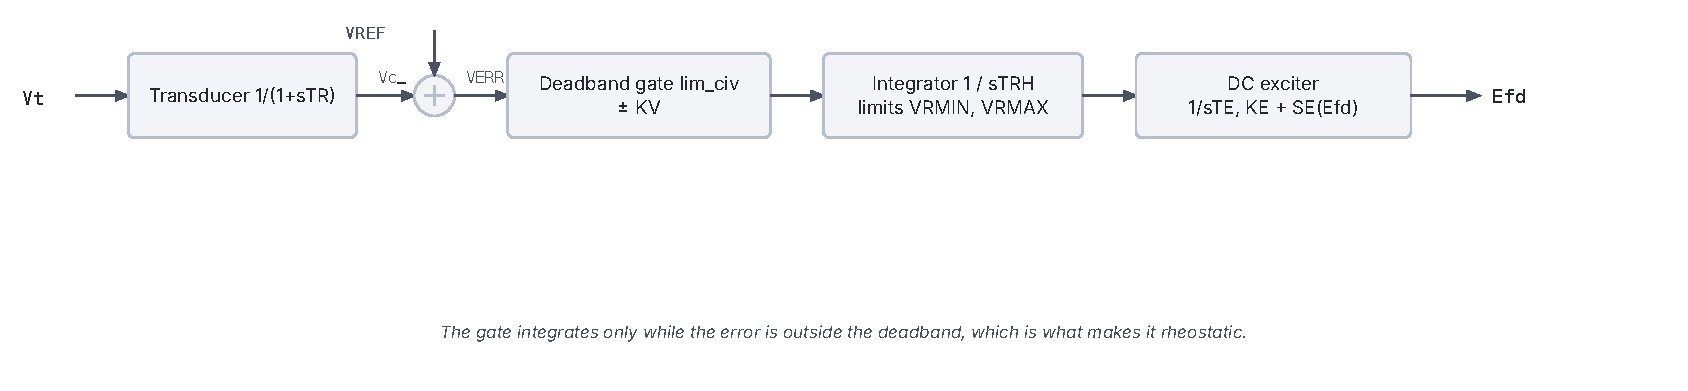
\includegraphics[width=0.98\linewidth]{figures/exc-ieeet5-light}
\caption{IEEET5 block diagram.}
\end{figure}

\subsubsection{Mathematical Description}\label{model-exc-ieee:mathematical-description-6}

\[V_{ERR} = V_{REF} - V_c\]

The integrator for rheostat position:

\[\dot{V}_{RH} = \frac{1}{T_{RH}} \cdot V_{ERR}, \quad V_{RMIN} \le V_{RH} \le V_{RMAX}\]

The \texttt{lim\_civ} block implements the deadband gating so that integration is active only when \(|V_{ERR}| > K_V\):

\[V_R = \begin{cases} V_{RMIN} & V_{ERR} < -K_V \\ V_{RH} & |V_{ERR}| \le K_V \\ V_{RMAX} & V_{ERR} > K_V \end{cases}\]

\[\dot{E}_{fd} = \frac{1}{T_E}\left[V_R - \left(K_E + S_E(E_{fd})\right) E_{fd}\right]\]

\subsubsection{Parameters}\label{model-exc-ieee:parameters-6}

\begin{small}\begin{longtable}[]{@{}lll@{}}
\toprule\noalign{}
Parameter & Description & Unit/Type \\
\midrule\noalign{}
\endhead
\bottomrule\noalign{}
\endlastfoot
\texttt{Kvcomp} & Voltage compensation gain & pu \\
\texttt{Rc} & Line drop resistance & pu \\
\texttt{Xc} & Line drop reactance & pu \\
\texttt{TRH} & Rheostat time & s \\
\texttt{KV} & Controller sensitivity deadband & pu \\
\texttt{VRMAX} & Maximum field voltage & pu \\
\texttt{VRMIN} & Minimum field voltage & pu \\
\texttt{TE} & Exciter integrator time constant & s \\
\texttt{KE} & Exciter self-excitation constant & pu \\
\texttt{E1} & Saturation point 1 & pu \\
\texttt{SE1} & Saturation factor at \(E_1\) & pu \\
\texttt{E2} & Saturation point 2 & pu \\
\texttt{SE2} & Saturation factor at \(E_2\) & pu \\
\end{longtable}\end{small}

\subsubsection{Variants}\label{model-exc-ieee:variants-6}

\begin{small}\begin{longtable}[]{@{}ll@{}}
\toprule\noalign{}
Model & Description \\
\midrule\noalign{}
\endhead
\bottomrule\noalign{}
\endlastfoot
\texttt{IEEET5} & Base model, non-continuously acting DC exciter \\
\end{longtable}\end{small}

\begin{center}\rule{0.5\linewidth}{0.5pt}\end{center}

\subsection{SEXS}\label{model-exc-ieee:sexs}

The SEXS (Simplified Excitation System) is a minimal two-parameter static exciter model from CIGR\'E publications, widely used for cases where detailed exciter data is unavailable. It has no measurement filter, no line drop compensation, and no rate feedback, just a lead-lag network and a limited first-order block.

\begin{figure}[htbp]
\centering
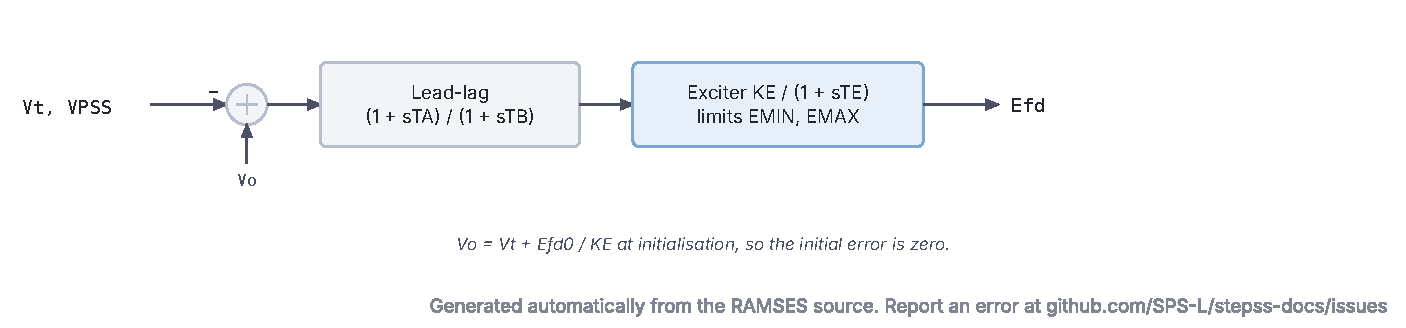
\includegraphics[width=0.98\linewidth]{figures/exc-sexs-light}
\caption{SEXS block diagram.}
\end{figure}

\subsubsection{Mathematical Description}\label{model-exc-ieee:mathematical-description-7}

\[\Delta V_{AVR} = V_t - V_o + V_{PSS}\]

\[G_{lag}(s) = \frac{1 + sT_A}{1 + sT_B}\]

\[E_{fd}(s) = G_{lag}(\Delta V_{AVR}) \cdot \frac{K_E}{1 + sT_E}, \quad E_{MIN} \le E_{fd} \le E_{MAX}\]

where \(V_o = V_t + E_{fd,0}/K_E\) is computed from initial conditions to achieve zero initial error.

\subsubsection{Parameters}\label{model-exc-ieee:parameters-7}

\begin{small}\begin{longtable}[]{@{}lll@{}}
\toprule\noalign{}
Parameter & Description & Unit/Type \\
\midrule\noalign{}
\endhead
\bottomrule\noalign{}
\endlastfoot
\texttt{TA} & Lead-lag numerator time constant & s \\
\texttt{TB} & Lead-lag denominator time constant & s \\
\texttt{KE} & Exciter gain & pu \\
\texttt{TE} & Exciter time constant & s \\
\texttt{EMIN} & Minimum field voltage & pu \\
\texttt{EMAX} & Maximum field voltage & pu \\
\end{longtable}\end{small}

\subsubsection{Variants}\label{model-exc-ieee:variants-7}

\begin{small}\begin{longtable}[]{@{}
  >{\raggedright\arraybackslash}p{(\linewidth - 4\tabcolsep) * \real{0.3350}}
  >{\raggedright\arraybackslash}p{(\linewidth - 4\tabcolsep) * \real{0.6650}}
@{}}
\toprule\noalign{}
\begin{minipage}[b]{\linewidth}\raggedright
Model
\end{minipage} & \begin{minipage}[b]{\linewidth}\raggedright
Description
\end{minipage} \\
\midrule\noalign{}
\endhead
\bottomrule\noalign{}
\endlastfoot
\texttt{SEXS} & Base simplified exciter \\
\texttt{SEXS\_IEEEST} & Adds IEEEST PSS (multi-mode: speed, power, or accelerating power input) \\
\texttt{SEXS\_STAB3\_lim} & Adds STAB3 PSS + integral OEL \\
\end{longtable}\end{small}

\subsubsection{Usage Example}\label{model-exc-ieee:usage-example-6}

\begin{Verbatim}
SYNC_MACH g1  g1  1. 1.  0.  0.   800. 760. 3. 0. 0.95
                    XT   0.15  1.1  0.25  0.2  0.7  *  0.2  0.1  6.0257  0.  5.00  0.05  *  0.1
              EXC SEXS   0.1 10.0 25.0 0.5 -5.0 5.0
              TOR CONSTANT ;
\end{Verbatim}

\section{ENTSO-E Models}\label{model-exc-ieee:entso-e-models}

\subsection{ENTSOE\_simp}\label{model-exc-ieee:entsoe_simp}

The ENTSO-E simplified exciter combines a built-in speed-signal PSS with a simple lead-lag AVR and first-order exciter block. It is the standard ENTSO-E model for dynamic studies where detailed exciter data is unavailable.

\begin{figure}[htbp]
\centering
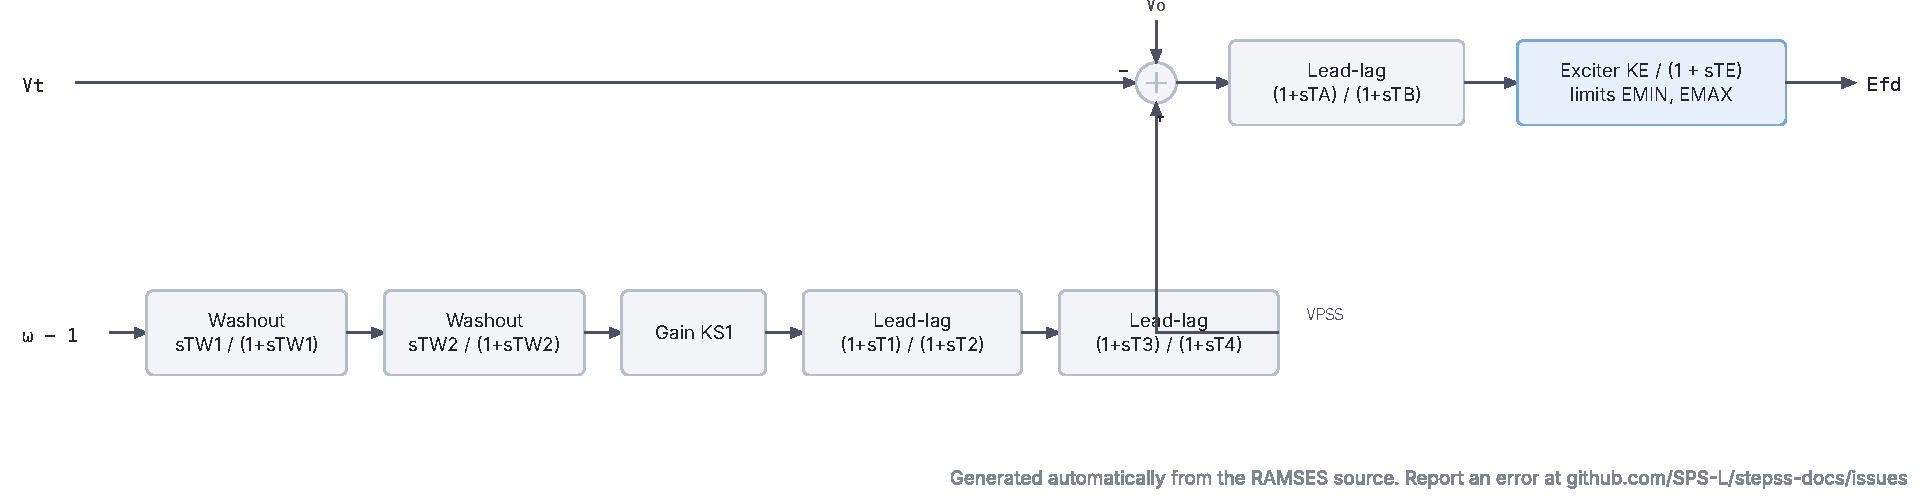
\includegraphics[width=0.98\linewidth]{figures/exc-entsoe-simp-light}
\caption{ENTSOE\_simp block diagram.}
\end{figure}

\subsubsection{Mathematical Description}\label{model-exc-ieee:mathematical-description-8}

The PSS (speed input \(\omega - 1\)) uses two washout stages and two lead-lag stages:

\[V_{PSS}(s) = (\omega - 1) \cdot \frac{sT_{W1}}{1+sT_{W1}} \cdot \frac{sT_{W2}}{1+sT_{W2}} \cdot K_{S1} \cdot \frac{1+sT_1}{1+sT_2} \cdot \frac{1+sT_3}{1+sT_4}\]

The AVR:

\[\Delta V_{AVR} = V_t - V_o + V_{PSS}\]

\[G_{lag}(s) = \frac{1 + sT_A}{1 + sT_B}\]

\[E_{fd}(s) = G_{lag}(\Delta V_{AVR}) \cdot \frac{K_E}{1 + sT_E}, \quad E_{MIN} \le E_{fd} \le E_{MAX}\]

\subsubsection{Parameters}\label{model-exc-ieee:parameters-8}

\begin{small}\begin{longtable}[]{@{}lll@{}}
\toprule\noalign{}
Parameter & Description & Unit/Type \\
\midrule\noalign{}
\endhead
\bottomrule\noalign{}
\endlastfoot
\texttt{TW1} & First washout time constant & s \\
\texttt{TW2} & Second washout time constant & s \\
\texttt{KS1} & PSS gain & pu \\
\texttt{T1} & First lead-lag numerator & s \\
\texttt{T2} & First lead-lag denominator & s \\
\texttt{T3} & Second lead-lag numerator & s \\
\texttt{T4} & Second lead-lag denominator & s \\
\texttt{VSTMIN} & PSS output lower limit & pu \\
\texttt{VSTMAX} & PSS output upper limit & pu \\
\texttt{TA} & AVR lead-lag numerator & s \\
\texttt{TB} & AVR lead-lag denominator & s \\
\texttt{KE} & Exciter gain & pu \\
\texttt{TE} & Exciter time constant & s \\
\texttt{EMIN} & Minimum field voltage & pu \\
\texttt{EMAX} & Maximum field voltage & pu \\
\end{longtable}\end{small}

\subsubsection{Variants}\label{model-exc-ieee:variants-8}

\begin{small}\begin{longtable}[]{@{}ll@{}}
\toprule\noalign{}
Model & Description \\
\midrule\noalign{}
\endhead
\bottomrule\noalign{}
\endlastfoot
\texttt{ENTSOE\_simp} & Base ENTSO-E simplified model with integrated PSS \\
\texttt{ENTSOE\_lim} & Adds integral OEL (same structure as \texttt{AC8B\_lim} OEL) \\
\end{longtable}\end{small}

\subsubsection{Usage Example}\label{model-exc-ieee:usage-example-7}

\begin{Verbatim}
SYNC_MACH g1  g1  1. 1.  0.  0.   800. 760. 3. 0. 0.95
                    XT   0.15  1.1  0.25  0.2  0.7  *  0.2  0.1  6.0257  0.  5.00  0.05  *  0.1
              EXC ENTSOE_simp   10.0 3.0 10.0 0.2 0.1 0.1 0.1 -0.05 0.05 0.05 0.1 25.0 1.0 -10.0 10.0
              TOR CONSTANT ;
\end{Verbatim}

\begin{center}\rule{0.5\linewidth}{0.5pt}\end{center}

\section{PSS Models}\label{model-exc-ieee:pss-models}

Power System Stabilizers (PSS) inject an additional signal \(V_{PSS}\) at the AVR summation point to damp electromechanical oscillations. All variants listed in the model index table include one of the PSS types described here.

\subsection{PSS2B: Dual-Input Stabilizer}\label{model-exc-ieee:pss2b-dual-input-stabilizer}

PSS2B accepts two input signals (typically speed \(\omega\) and electrical power \(P_e\)) and processes them through independent washout chains before combining. It corresponds to IEEE Std 421.5-2016 Type PSS2B.

\begin{docsnote}{Differences from other vendors' PSS2B}

Implementations of PSS2B vary, so parameter lists do not transfer between tools unchanged. Three differences are worth knowing when porting data in:

\begin{itemize}
\tightlist
\item
  RAMSES names the two transducer lags \(T_6\) and \(T_7\), following IEEE 421.5. Some tools name the same two constants \(T_{W6}\) and \(T_{W7}\), which is easy to misread as a third and fourth washout.
\item
  RAMSES has no \(K_{S4}\) and no ramp-tracking filter (\(AA\), \(T_A\), \(T_B\)). Data sets carrying those come from an extended PSS2B and cannot be transferred field by field.
\item
  RAMSES adds a leading \texttt{speedinput} selector that chooses the speed signal source. It has no counterpart elsewhere and must be supplied as the first stabiliser parameter.
\end{itemize}

\end{docsnote}

\[V_{S1} = \text{clamp}(VSI_1, V_{S1MIN}, V_{S1MAX})\]

Channel 1 (input 1 washout):

\[V_{S1} \xrightarrow{sT_{W1}/(1+sT_{W1})} \xrightarrow{sT_{W2}/(1+sT_{W2})} \xrightarrow{1/(1+sT_6)} pss_{3}\]

Channel 2 (input 2 washout):

\[V_{S2} \xrightarrow{sT_{W3}/(1+sT_{W3})} \xrightarrow{sT_{W4}/(1+sT_{W4})} \xrightarrow{K_{S2}/(1+sT_7)} pss_{6}\]

Combination and lead-lag chain (variant M=5, N=1 implemented):

\[pss_7 = pss_3 - K_{S3} \cdot pss_6\]

\[pss_7 \xrightarrow{(1+sT_8)/(1+sT_9)} \xrightarrow{1/(1+sT_9)^4} pss_{12}\]

\[pss_{13} = pss_{12} + pss_6\]

\[pss_{13} \xrightarrow{K_{S1}(1+sT_1)/(1+sT_2)} \xrightarrow{(1+sT_3)/(1+sT_4)} \xrightarrow{(1+sT_{10})/(1+sT_{11})} V_{PSS}\]

\[V_{PSS} = \text{clamp}(V_{PSS,unlim}, V_{STMIN}, V_{STMAX})\]

\textbf{PSS2B Parameters (additional to base exciter):}

\begin{small}\begin{longtable}[]{@{}ll@{}}
\toprule\noalign{}
Parameter & Description \\
\midrule\noalign{}
\endhead
\bottomrule\noalign{}
\endlastfoot
\texttt{speedinput} & Input selection (1=speed+power, 2=power+speed) \\
\texttt{TW1}, \texttt{TW2} & Channel 1 washout time constants \\
\texttt{T6} & Channel 1 filter \\
\texttt{TW3}, \texttt{TW4} & Channel 2 washout time constants \\
\texttt{T7}, \texttt{KS2} & Channel 2 filter gain and time constant \\
\texttt{KS3} & Channel coupling gain \\
\texttt{T8}, \texttt{T9} & Ramp-tracking filter \\
\texttt{KS1} & Overall PSS gain \\
\texttt{T1}--\texttt{T4}, \texttt{T10}, \texttt{T11} & Lead-lag time constants \\
\texttt{VS1MIN}, \texttt{VS1MAX} & Input 1 limits \\
\texttt{VS2MIN}, \texttt{VS2MAX} & Input 2 limits \\
\texttt{VSTMIN}, \texttt{VSTMAX} & Output limits \\
\end{longtable}\end{small}

\begin{center}\rule{0.5\linewidth}{0.5pt}\end{center}

\begin{figure}[htbp]
\centering
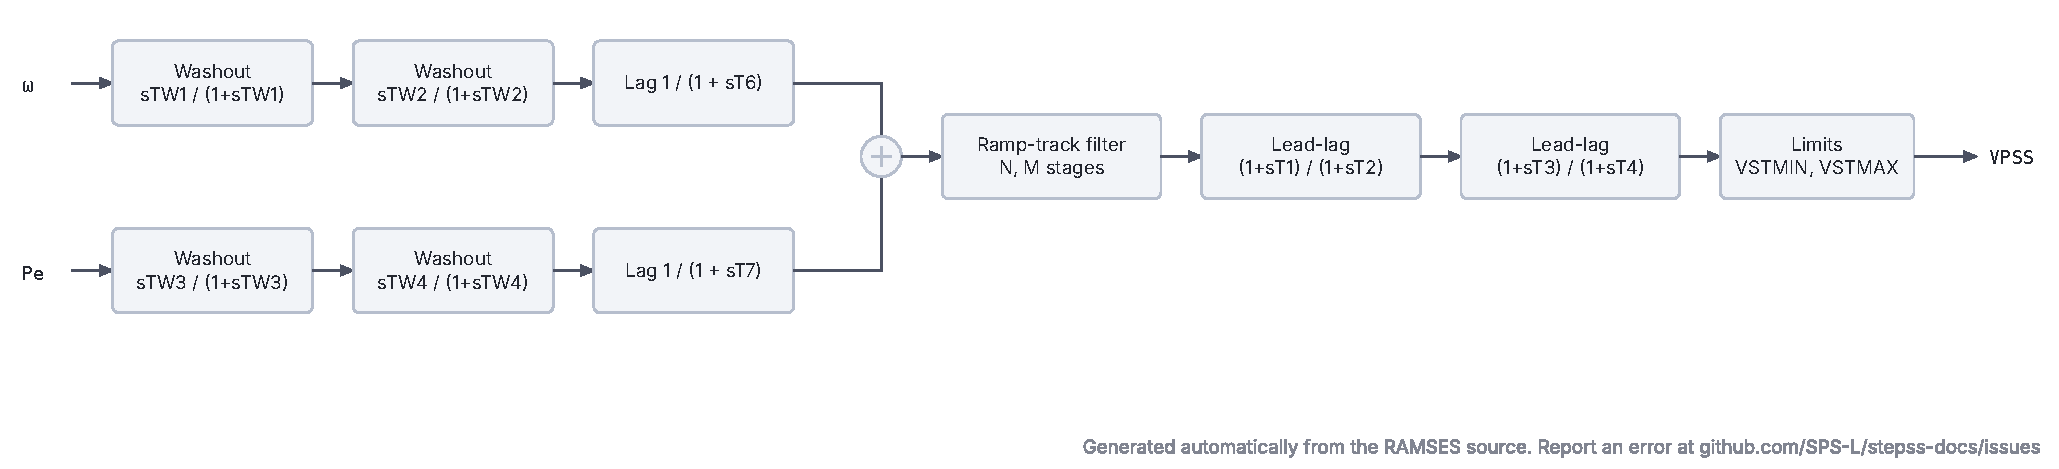
\includegraphics[width=0.98\linewidth]{figures/pss-pss2b-light}
\caption{PSS2B block diagram.}
\end{figure}

\subsection{PSS3B: Two-Input Second-Order Filter Stabilizer}\label{model-exc-ieee:pss3b-two-input-second-order-filter-stabilizer}

PSS3B processes two input channels through measurement filters and washout stages, then combines them and applies two cascaded second-order lead-lag filters. It corresponds to IEEE Std 421.5-2016 Type PSS3B.

\[V_{SI1} \xrightarrow{1/(1+sT_1)} \xrightarrow{K_{S1} sT_{W1}/(1+sT_{W1})} pss_2\]

\[V_{SI2} \xrightarrow{1/(1+sT_2)} \xrightarrow{K_{S2} sT_{W2}/(1+sT_{W2})} pss_4\]

\[pss_5 = pss_2 - pss_4\]

\[pss_5 \xrightarrow{K_S sT_{W3}/(sT_{W4}+1)} pss_6\]

\[pss_6 \xrightarrow{\text{TF1: } \frac{A_2 + sA_1 + s^2/A_4}{A_4 + sA_3 + s^2/A_4}} \xrightarrow{\text{TF2: } \frac{A_6+sA_5+s^2/A_8}{A_8+sA_7+s^2/A_8}} V_{PSS}\]

\[V_{PSS} = \text{clamp}(V_{PSS,unlim}, V_{STMIN}, V_{STMAX})\]

\textbf{PSS3B Parameters (additional):}

\begin{small}\begin{longtable}[]{@{}ll@{}}
\toprule\noalign{}
Parameter & Description \\
\midrule\noalign{}
\endhead
\bottomrule\noalign{}
\endlastfoot
\texttt{speedinput} & Input mode selection \\
\texttt{T1}, \texttt{KS1}, \texttt{TW1} & Channel 1 filter, gain, washout \\
\texttt{T2}, \texttt{KS2}, \texttt{TW2} & Channel 2 filter, gain, washout \\
\texttt{KS}, \texttt{TW3}, \texttt{TW4} & Combined washout gain and time constants \\
\texttt{A1}--\texttt{A8} & Second-order filter coefficients \\
\texttt{VSTMIN}, \texttt{VSTMAX} & Output limits \\
\end{longtable}\end{small}

\begin{center}\rule{0.5\linewidth}{0.5pt}\end{center}

\begin{figure}[htbp]
\centering
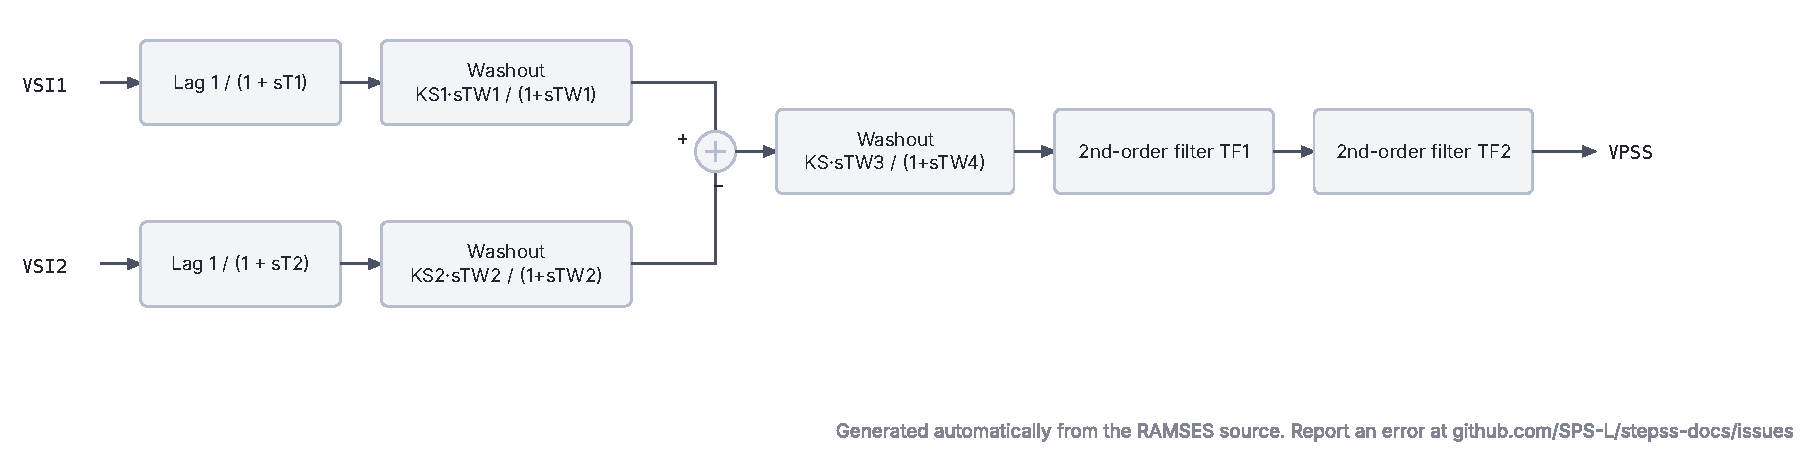
\includegraphics[width=0.98\linewidth]{figures/pss-pss3b-light}
\caption{PSS3B block diagram.}
\end{figure}

\subsection{PSS4B: Three-Band Multi-Input Stabilizer}\label{model-exc-ieee:pss4b-three-band-multi-input-stabilizer}

PSS4B is a three-band stabilizer that separates the speed deviation signal into low-, intermediate-, and high-frequency components. Each band uses a pair of lead-lag filters. This model corresponds to IEEE Std 421.5-2016 Type PSS4B.

The speed signal \(\Delta\omega = \omega - 1\) passes through a digital transducer (\texttt{tf2p2z}) to obtain the low/intermediate input. Electrical power \(P_e\) passes through two washouts and a low-pass filter to derive the high-frequency component \(\Delta\omega_H\).

\textbf{Low-frequency band} (\(\Delta\omega_{L-I}\) input):

\[pss_4 = \Delta\omega_{L-I} \cdot \frac{K_{L1}(K_{L11} + sT_{L1})}{1 + sT_{L2}}\]

\[pss_5 = \Delta\omega_{L-I} \cdot \frac{K_{L2}(K_{L17} + sT_{L7})}{1 + sT_{L8}}\]

\[V_{PSSL} = \text{clamp}\!\left(K_L(pss_4 - pss_5),\, V_{LMin}, V_{LMax}\right)\]

\textbf{Intermediate-frequency band} (same \(\Delta\omega_{L-I}\) input):

\[V_{PSSI} = \text{clamp}\!\left(K_I(pss_7 - pss_8),\, V_{IMin}, V_{IMax}\right)\]

\textbf{High-frequency band} (\(\Delta\omega_H\) input):

\[V_{PSSH} = \text{clamp}\!\left(K_H(pss_{10} - pss_{11}),\, V_{HMin}, V_{HMax}\right)\]

\[V_{PSS} = \text{clamp}(V_{PSSL} + V_{PSSI} + V_{PSSH},\, V_{STMin}, V_{STMax})\]

\textbf{PSS4B Parameters (additional):}

\begin{small}\begin{longtable}[]{@{}ll@{}}
\toprule\noalign{}
Parameter & Description \\
\midrule\noalign{}
\endhead
\bottomrule\noalign{}
\endlastfoot
\texttt{H} & Generator inertia constant (for high-freq path) \\
\texttt{KL1}, \texttt{KL11}, \texttt{TL1}, \texttt{TL2} & Low-band filter 1 \\
\texttt{KL2}, \texttt{KL17}, \texttt{TL7}, \texttt{TL8} & Low-band filter 2 \\
\texttt{KL}, \texttt{VLMax}, \texttt{VLMin} & Low-band gain and limits \\
\texttt{KI1}, \texttt{KI11}, \texttt{TI1}, \texttt{TI2} & Intermediate-band filter 1 \\
\texttt{KI2}, \texttt{KI17}, \texttt{TI7}, \texttt{TI8} & Intermediate-band filter 2 \\
\texttt{KI}, \texttt{VIMax}, \texttt{VIMin} & Intermediate-band gain and limits \\
\texttt{KH1}, \texttt{KH11}, \texttt{TH1}, \texttt{TH2} & High-band filter 1 \\
\texttt{KH2}, \texttt{KH17}, \texttt{TH7}, \texttt{TH8} & High-band filter 2 \\
\texttt{KH}, \texttt{VHMax}, \texttt{VHMin} & High-band gain and limits \\
\texttt{VSTMax}, \texttt{VSTMin} & Total output limits \\
\end{longtable}\end{small}

\begin{center}\rule{0.5\linewidth}{0.5pt}\end{center}

\begin{figure}[htbp]
\centering
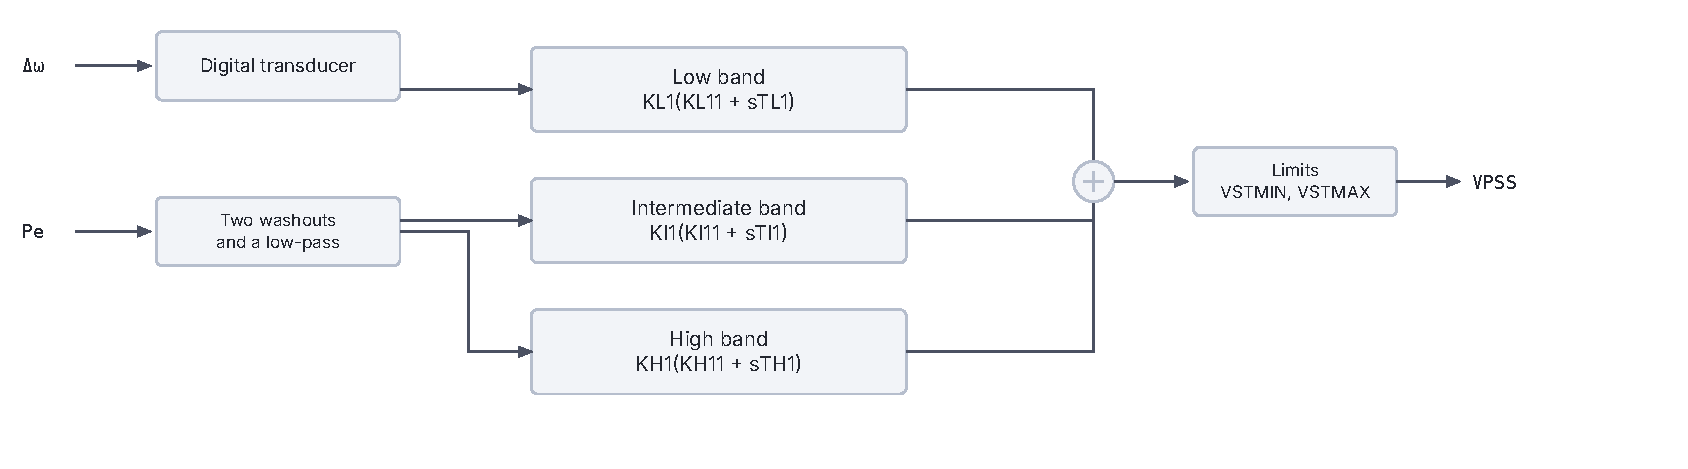
\includegraphics[width=0.98\linewidth]{figures/pss-pss4b-light}
\caption{PSS4B block diagram.}
\end{figure}

\subsection{IEEEST: Single-Input Stabilizer}\label{model-exc-ieee:ieeest-single-input-stabilizer}

The IEEEST is a general-purpose single-input PSS with selectable input signal (speed deviation, electrical power, or computed accelerating power). It corresponds to IEEE Std 421.5-2016 Type PSS1A. Two second-order lead-lag filters provide frequency shaping before two first-order lead-lags and a washout stage.

\[VS_1 \xrightarrow{\frac{1}{A_2 + sA_1 + s^2/(A_1 A_2)}} \xrightarrow{\frac{A_6 + sA_5 + s^2/(A_3 A_4)}{A_4 + sA_3 + s^2/(A_3 A_4)}} VS_3\]

\[VS_3 \xrightarrow{\frac{1+sT_1}{1+sT_2}} \xrightarrow{\frac{1+sT_3}{1+sT_4}} \xrightarrow{\frac{K_S sT_5/T_6}{1+sT_6}} V_{PSS}\]

\[V_{PSS} = \text{clamp}(V_{PSS,unlim}, V_{LSMIN}, V_{LSMAX})\]

Input selection (\texttt{speedinput}): 1 = rotor speed deviation, 3 = electrical power, 4 = computed accelerating power (\(2H \, d\omega/dt\)).

\textbf{IEEEST Parameters (additional):}

\begin{small}\begin{longtable}[]{@{}ll@{}}
\toprule\noalign{}
Parameter & Description \\
\midrule\noalign{}
\endhead
\bottomrule\noalign{}
\endlastfoot
\texttt{speedinput} & Input mode (1, 3, or 4) \\
\texttt{A1}--\texttt{A6} & Second-order filter coefficients \\
\texttt{T1}--\texttt{T6} & Lead-lag and washout time constants \\
\texttt{KS} & Overall PSS gain \\
\texttt{LSMIN}, \texttt{LSMAX} & Output limits \\
\texttt{KS4} & Inertia constant for accelerating power (= 2H) \\
\texttt{TW4} & Derivative filter time constant \\
\end{longtable}\end{small}

\begin{center}\rule{0.5\linewidth}{0.5pt}\end{center}

\begin{figure}[htbp]
\centering
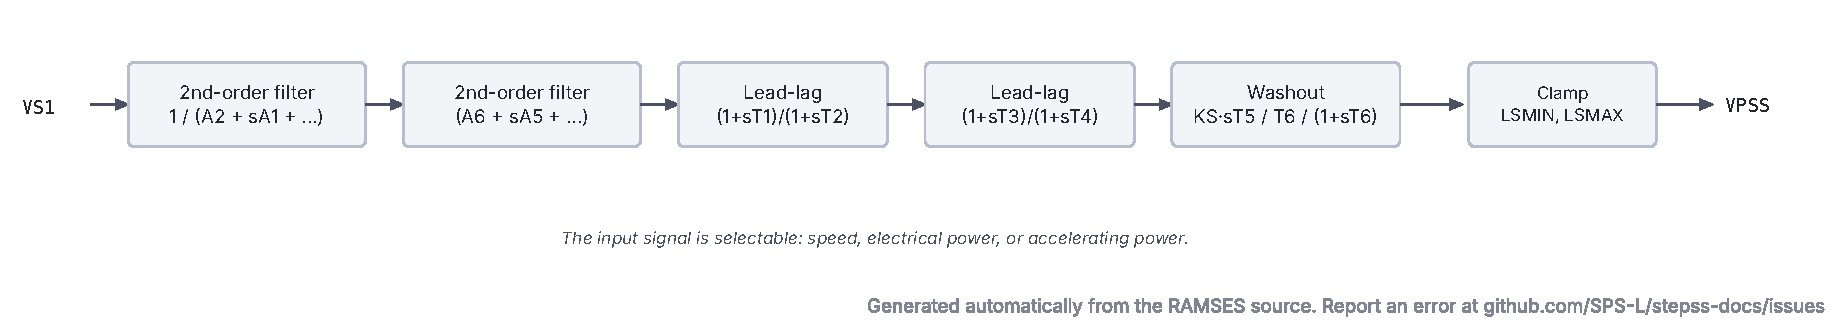
\includegraphics[width=0.98\linewidth]{figures/pss-ieeest-light}
\caption{IEEEST block diagram.}
\end{figure}

\subsection{STAB3: Power-Input Stabilizer}\label{model-exc-ieee:stab3-power-input-stabilizer}

The STAB3 is a simplified PSS that takes electrical power \(P_e\) as input, applies two sequential first-order filters and a washout-type derivative block, producing a stabilizing signal.

\[P_e \xrightarrow{1/(1+sT_t)} stab_1 \xrightarrow{1/(1+sT_{X1})} stab_2 \xrightarrow{-K_X s/(1+sT_{X2})} stab_3\]

\[V_{PSS} = \text{clamp}(stab_3, -V_{LIM}, V_{LIM})\]

\textbf{STAB3 Parameters:}

\begin{small}\begin{longtable}[]{@{}ll@{}}
\toprule\noalign{}
Parameter & Description \\
\midrule\noalign{}
\endhead
\bottomrule\noalign{}
\endlastfoot
\texttt{Tt} & Input measurement time constant \\
\texttt{TX1} & First filter time constant \\
\texttt{KX} & Stabilizer gain \\
\texttt{TX2} & Washout time constant \\
\texttt{VLIM} & Output limit \\
\end{longtable}\end{small}

\begin{center}\rule{0.5\linewidth}{0.5pt}\end{center}

\section{OEL and Limiter Models}\label{model-exc-ieee:oel-and-limiter-models}

Over-Excitation Limiters (OEL) prevent sustained field current overloads that would thermally damage the field winding. They generate a signal \(V_{OEL}\) that reduces the AVR output when field current exceeds thermal limits.

\begin{figure}[htbp]
\centering
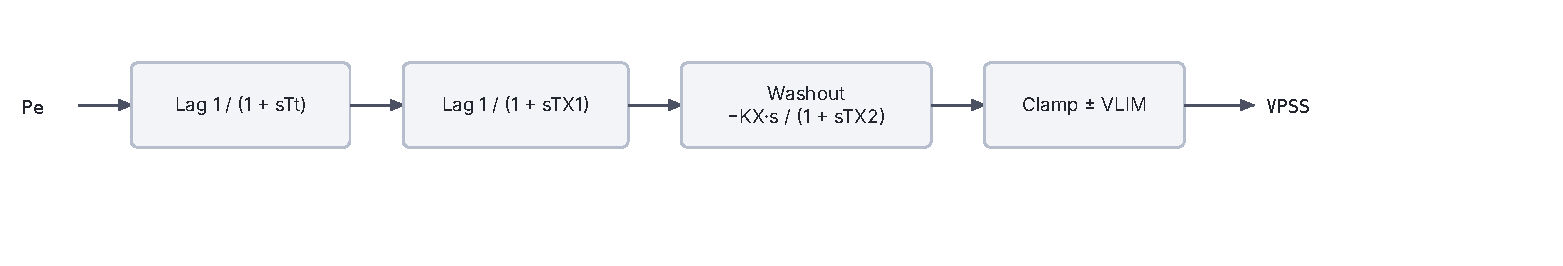
\includegraphics[width=0.98\linewidth]{figures/pss-stab3-light}
\caption{STAB3 block diagram.}
\end{figure}

\subsection{MAXEX2: Field Current Limiter with Timer and Hysteresis}\label{model-exc-ieee:maxex2-field-current-limiter-with-timer-and-hysteresis}

The MAXEX2 is a field current limiter derived from IEEE work, using a simplified three-point piece-wise linear timer It is designed for the EXST1/ST1A topology where the OEL output is injected at the reference summation point (not the LV gate).

\textbf{Timer phase:} The measured current \(I_{fd,mes}\) (selected as either field current or \(E_{fd}\) via parameter \texttt{IC}) drives a \texttt{timer3} block with three \((I_{fd}, T)\) operating points. The \texttt{hyst} block latches when timer \ensuremath{\ge} 1.

\textbf{Integral phase:} Once latched, the error drives a limited integrator:

\[e_{IFD} = I_{fd,ref} - I_{fd,mes}\]

\[\dot{V}_{OEL} = \frac{e_{IFD}}{K_{MX}}, \quad V_{LOW} \le V_{OEL} \le 0\]

\(V_{OEL}\) is subtracted from the reference (\(V_{REF} - V_{OEL}\), i.e.~Negative reduces reference).

\textbf{MAXEX2 Parameters:}

\begin{small}\begin{longtable}[]{@{}ll@{}}
\toprule\noalign{}
Parameter & Description \\
\midrule\noalign{}
\endhead
\bottomrule\noalign{}
\endlastfoot
\texttt{IC} & Input selection: 0 = \(E_{fd}\), 1 = \(I_{fd}\) \\
\texttt{IFDrated} & Rated field current (reference) \\
\texttt{IFD1}, \texttt{TIME1} & Timer point 1 (current level, allowable duration) \\
\texttt{IFD2}, \texttt{TIME2} & Timer point 2 \\
\texttt{IFD3}, \texttt{TIME3} & Timer point 3 \\
\texttt{IFDDES} & Desired steady-state field current after limiting \\
\texttt{KMX} & Integrator time constant inverse (1/KMX = integration rate) \\
\texttt{VLOW} & Lower limit of OEL output (e.g.~\ensuremath{-}1.0 pu) \\
\end{longtable}\end{small}

\begin{center}\rule{0.5\linewidth}{0.5pt}\end{center}

\begin{figure}[htbp]
\centering
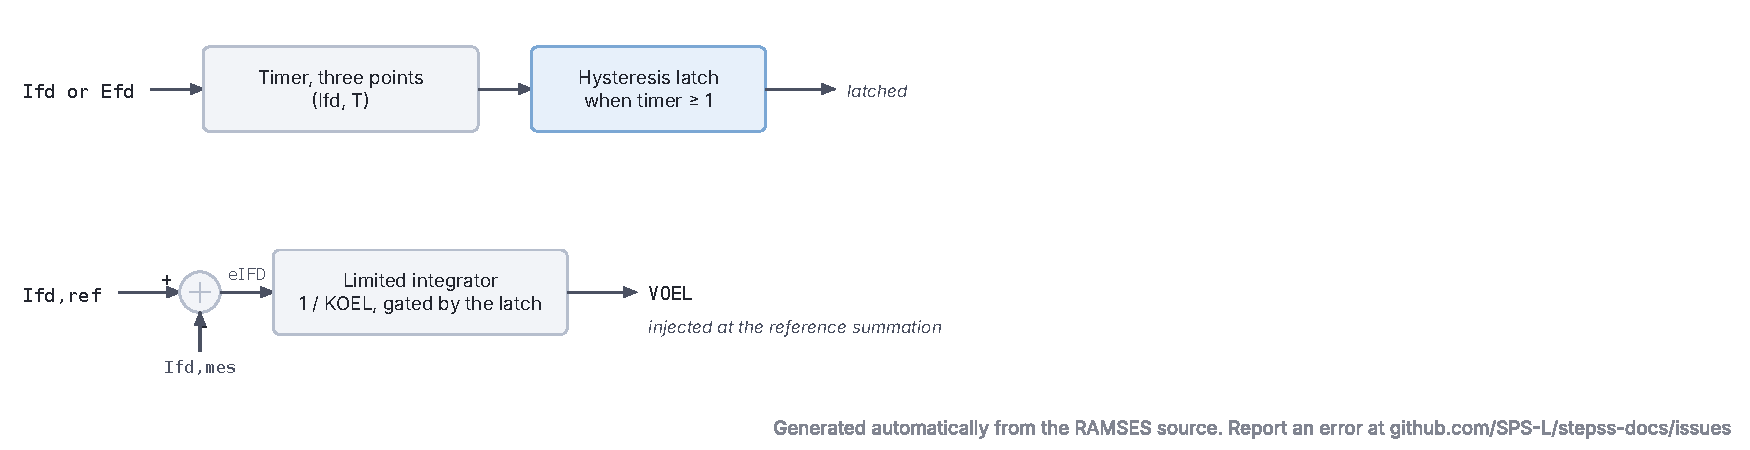
\includegraphics[width=0.98\linewidth]{figures/exc-maxex2-light}
\caption{MAXEX2 block diagram.}
\end{figure}

\subsection{Integral OEL (\_lim variants)}\label{model-exc-ieee:integral-oel-_lim-variants}

The simple integral OEL used in \texttt{AC8B\_lim}, \texttt{ST1A\_lim}, \texttt{SEXS\_STAB3\_lim}, and \texttt{ENTSOE\_lim} variants computes the over-excitation signal through a clamped integrator acting on the difference between measured field current and \(1.05 \cdot I_{FDN}\), with an input clamp at \(0.35 \cdot I_{FDN}\).

\[\Delta I_{fd,1} = I_{fd} - 1.05 \cdot I_{FDN}\]

\[\Delta I_{fd,2} = \min(\Delta I_{fd,1},\, 0.35 \cdot I_{FDN})\]

\[\dot{x}_{OEL} = \frac{\Delta I_{fd,2}}{T_{OEL}}, \quad L_{OEL} \le x_{OEL} \le U_{OEL}\]

\[V_{OEL} = \text{clamp}(K_{OEL} \cdot x_{OEL},\, OEL_{LI},\, 0)\]

A stator current limiter (SCL) with analogous structure acts on \(I_{st} = \sqrt{P^2 + Q^2}/V_t\) relative to \(1.025 \cdot I_{GN}\).

\textbf{Integral OEL Parameters (in \_lim variants):}

\begin{small}\begin{longtable}[]{@{}ll@{}}
\toprule\noalign{}
Parameter & Description \\
\midrule\noalign{}
\endhead
\bottomrule\noalign{}
\endlastfoot
\texttt{IFDN} & Nominal field current (OEL trigger at 1.05\ensuremath{\times}) \\
\texttt{TOEL} & OEL integrator time constant \\
\texttt{LOEL} & OEL integrator lower limit \\
\texttt{UOEL} & OEL integrator upper limit \\
\texttt{KOEL} & OEL output gain \\
\texttt{OELLI} & OEL output lower limit \\
\texttt{IGN} & Nominal stator current (SCL trigger at 1.025\ensuremath{\times}) \\
\texttt{TSCL} & SCL integrator time constant \\
\texttt{LSCL} & SCL integrator lower limit \\
\texttt{USCL} & SCL integrator upper limit \\
\texttt{KSCL} & SCL output gain \\
\texttt{SCLLI} & SCL output lower limit \\
\end{longtable}\end{small}

\begin{center}\rule{0.5\linewidth}{0.5pt}\end{center}

For full documentation of the CODEGEN DSL primitives used in these models (\texttt{tf1p}, \texttt{tf1p1z}, \texttt{tf1plim}, \texttt{inlim}, \texttt{pictl}, etc.), see the \hyperref[ch-libray_blocks]{CODEGEN Blocks} reference.

\begin{figure}[htbp]
\centering
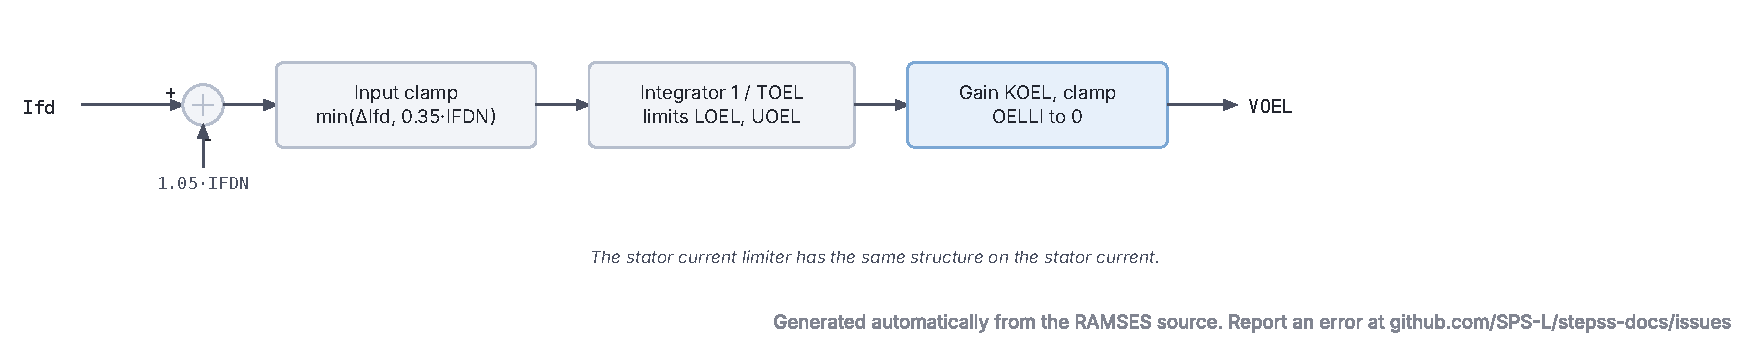
\includegraphics[width=0.98\linewidth]{figures/exc-integral-oel-light}
\caption{Integral over-excitation limiter block diagram.}
\end{figure}
